%%
%% Beginning of file 'siggma.tex'
%%
%% Created March 17 2017 by LB
%%
%% This is a manuscript for the siggma data release paper using the
%% AASTeX v6.1 LaTeX 2e macros.
%%
\documentclass[manuscript]{aastex61}
%%%%%%%%%%%%%%%%%%%%%%%%%%%%%%%%%%%%%%%%%%%%%%%%%%%%%%%%%%%%%%%%%%%%%%%%%%%%%%%%

\hypersetup{linkcolor=red,citecolor=blue,filecolor=cyan,urlcolor=magenta}

%\received{}
%\revised{}
%\accepted{}
%\submitjournal{}

\shorttitle{SIGGMA. II}
\shortauthors{Liu et al.}
\watermark{DRAFT}
\setwatermarkfontsize{100 pt}

%\usepackage[a4paper, margin=1.7cm]{geometry}
\usepackage[flushleft]{threeparttable}
\usepackage{graphicx}
\usepackage[caption = false]{subfig}
\usepackage{float}
\usepackage{longtable}
\newcommand{\hii}{{\rm H\,}{{\sc ii}}}
\newcommand{\hi}{{\rm H\,}{{\sc i}}}
\newcommand{\kms}{\,km\,s$^{-1}$}
\newcommand{\kpc}{\,kpc}
\newcommand{\ghz}{\,GHz}
\newcommand{\um}{\mu m}
%%%%%%%%%%%%%%%%%%%%%%%%%%%%%%%%%%%%%%%%%%%%%%%%%%%%%%%%%%%%%%%%%%%%%%%%%%%%%%%%
\begin{document}

\title{Survey of Ionized Gas of the Galaxy, Made with the Arecibo telescope (SIGGMA): Inner Galaxy Data Release}

\correspondingauthor{Bin Liu}
\email{bliu@mail.wvu.edu}
\author[0000-0002-1311-8839]{Bin Liu}
\affil{National Astronomical Observatories, Chinese Academy of Sciences, Beijing 100012, China}
\affil{West Virginia University, Morgantown, WV 26506, USA}
\author{L. D. Anderson}
\affil{West Virginia University, Morgantown, WV 26506, USA}
\affil{Adjunct Astronomer at the Green Bank Observatory, P.O. Box 2, Green Bank WV 24944, USA}
\affil{Center for Gravitational Waves and Cosmology, West Virginia University, Chestnut Ridge Research Building, Morgantown, WV 26505,
USA}
\author{Travis Mclntyre}
\affil{University of New Mexico, Albuquerque, NM 87131, USA}
\author{D. Anish Roshi}
\affil{National Radio Astronomy Observatory, Green Bank \& Charlottesville, VA 22903, USA}
\author{Ed Churchwell}
\affil{University of Wisconsin-Madison, Madison, WI 53706, USA}
\author{Robert Minchin}
\affil{Arecibo Observatory, HC03 Box 53995, Arecibo 00612, Puerto Rico}
%\author{M. Lebron}
%\affil{University of Puerto Rico, PO Box 23323, San Juan 00931, Puerto Rico}
\author{Yervant Terzian}
\affil{Cornell University, Ithaca, NY 14853, USA}

\begin{abstract}
The Survey of Ionized Gas of the Galaxy, Made with the Arecibo telescope (SIGGMA) provides a fully-sampled view of the radio recombination line (RRL) emission from the portion of the Galactic plane visible by Arecibo.
Observations use the Arecibo L-band Feed Array (ALFA), with a FWHM beam size of 3.4$\arcmin$ and a spectral resolution of 5.1\kms.
Twelve hydrogen RRLs from H163$\alpha$ to H174$\alpha$ are located within the 300~MHz instantaneous bandpass, which extends from 1225 MHz to 1525 MHz.
The principle data products are cubes of average (``stacked'') RRL emission, which we provide here for the inner Galaxy region $32\degr \le \ell \le 70 \degr$, $|b| \le 1.5\degr$.
The stacked RRL spectral rms per beam at the native 5.1\kms\ velocity resolution is $\sim 0.65$\,mJy\,beam$^{-1}$, making this the most sensitive large-scale fully-sampled RRL survey extant.
SIGGMA is sensitive to discrete \hii\ regions and diffuse ionized gas.
We catalogue 338 RRL detections of RRL emission toward known \hii\ regions from the {\it WISE} catalog of Galactic \hii\ Regions, 
 as well as toward 84 \hii\ region candidates from this catalog. 
We identify 11 Carbon RRL emission regions, all of which are spatially coincident with known \hii\ regions.  Carbon RRLs are thought to arise from \hii\ region photo-dissociation regions (PDRs), and these bright regions represent excellent candidates for future study of PDR radiation. 
We detect RRL emission from 14 of the 32 supernova remnants (SNRs) found in the survey area.
The velocities derived from these regions give kinematic distances in agreement with those found in the literature.  Future RRL observations of SNRs may therefore help in determining their distances.
Finally, we analyze the two bright star-forming complexes, W49 and W51.
We report two diffuse RRL emission components separated by velocities with respect to local standard of rest (LSR) within the W49 region.
The map of W51 shows the RRL emitting gas morphology matches with that of the infrared emission.  
Moreover, there is are also diffuse ionized gas emission from where the infrared emission is not obvious, implying that the RRL emission may be due to leaking photons from \hii\ regions.LDA: need to mention data being released, with pixel size

\end{abstract}

\keywords{radio lines: ISM --- \hii\ regions --- catalogs --- surveys}

\section{Introduction} \label{sec_intr}
%1. RRL in general.
Radio recombination lines (RRLs) are ideal tracers of the ionized interstellar medium (ISM).
In contrast to observations at optical and infrared (IR) wavelengths, RRLs are essentially unaffected by interstellar extinction.  They therefore provide us with a probe of ionized gas in the Galactic plane, sampling the emission from \hii\ regions, photo-dissociation regions (PDRs), planetary nebulae (PNe), supernova remnants (SNRs), and diffuse ionized gas.  From the observed RRL parameters, one can derive the physical properties of the emitting regions, such as the electron temperature, the gas kinematics, and information about thermal and turbulent motions.

%2. Other RRLs surveys.
There have been many pointed RRL surveys of individual Galactic \hii\ regions, beginning in the 1970s \citep[e.g.][]{Reifenstein1970,Wilson1970}.
\citet{Lockman1989} cataloged 462 \hii\ regions in the northern sky by observing RRLs at 3cm wavelength towards Galactic continuum sources.
\citet{Caswell1987} carried out a comprehensive \hii\ survey of 316 \hii\ regions in the southern sky using H109$\alpha$ \& H110$\alpha$.
The Green Bank Telescope (GBT) \hii\ Region Discovery Survey \citep[GBT HRDS;][]{Bania2010,Anderson2011,Anderson2015b} is the most recent RRL survey of targeted sources.
Its sample was selected by examining the IR and radio emission of candidate \hii\ regions. 
The HDRS has doubled the number of known \hii\ regions north of $\delta=-45\degr$, which is $340\degr \leq \ell \leq 240\degr$ at $b = 0\degr$.

In addition to emission from discrete \hii\ regions around massive stars, RRLs also trace the emission from low-density diffuse ionized gas (\textless1 cm$^{-3}$), referred to as the warm ($T_e \sim 3000 - 8000$ K) ionized medium (WIM), pervades the Galactic disk.
This component has a scale height of $\sim$1000\,pc and is usually studied using optical recombination lines and pulsar dispersion measures \citep{Taylor1977,Reynolds1990}.
%SIGGMA can study WIM with RRLs, at higher spacial resolution than that of previous studies \citep{Alves2015}. 
LDA: Other papers?

% RRL maps
There are few unbiased surveys of mapped RRL emission.
\citet{Alves2010,Alves2012,Alves2015} used RRLs within the bandpass of the \hi\ Parkes All-Sky Survey \citep[HIPASS;][]{Staveley1996}, which covers from $\ell=196\degr$ to $\ell=360\degr$ in the fourth quadrant, and from $\ell = 0\degr$ to $\ell = 52\degr$ in the first quadrant, both within $|b| \leq 5\degr$.
They observed H166$\alpha$, H167$\alpha$, and H168$\alpha$ at L-band with a spatial resolution of $14.4\arcmin$ and a velocity resolution of 20\kms.  Their typical rms noise in the stacked spectra is 4.5 mK (6.4 mJy\,beam$^{-1}$).
The HI/OH/RRL survey with the Very Large Array \citep[THOR;][]{Beuther2016} also produced RRL maps, with a smoothed angular resolution of $40\arcsec$ and a velocity resolution of 10\kms. Their rms noise is $\sim$2.3 mJy\,beam$^{-1}$ by stacking 10 RRLs.
Being an interferometric survey, the THOR RRL data are not sensitive to emission from diffuse ionized gas.
%%%%%%%%%%%%%%%%%%%%%%%%%%%%%%%%%%%%%%%%%%%%%%%%%%%%%
%Comparison of RMS OF SIGGMA WITH THAT OF THOR
%  = STACK_SPEC_RMS * BEAM^2 * CHANNEL_RES^0.5
%         BEAM   CHANNEL_RES    STACK_SPEC_RMS      RATIO
%SIGGMA   3'.4    4.2 KM/S       0.65 MJY/BEAM       15
%THOR     40"     10 KM/S        2.3  MJY/BEAM       3
%HIPASS   14'.4   20 KM/S        6.4  MJY/BEAM       5935
%%%%%%%%%%%%%%%%%%%%%%%%%%%%%%%%%%%%%%%%%%%%%%%%%%%%%

%3. SIGGMA motivation.
We introduced the Survey of Ionized Gas in the Galaxy, made with the Arecibo Telescope (SIGGMA) in \citet[hereafter ``Paper I'']{Liu2013}.
SIGGMA is a radio recombination line (RRL) survey at 1.4 GHz that is fully sampling the entire Galactic plane observable with the 305-m William E. Gordon Telescope at the Arecibo Observatory.
With an rms noise of $\sim$1\,mJy\,beam$^{-1}$, SIGGMA remains the most sensitive fully-sampled RRL survey.

%4. Purpose of this paper.
In this paper, we present SIGGMA data from the inner Galaxy ($32 \degr \leq l \leq 70 \degr$).
These inner-Galaxy data were collected commensally with the Arecibo pulsar survey ``PALFA'' \citep{Cordes2006, Lazarus2015}.
In the outer Galaxy ($175 \degr \leq l \leq 207 \degr $), SIGGMA is observed commensally with the ALFA zone of avoidance (ZOA) survey \citep[][]{McIntyre2015}, which is still ongoing.
The survey data from the outer Galaxy will be discussed in a future paper. 
We describe the SIGGMA observations and data reduction in Section~\ref{sec_obs_data}.
Section\,\ref{sec_cata} gives the \hii\ region catalogues as the initial results of the survey. 
The distribution of RRL emission and derived free-free emission along the Galactic disk are present in Section\,\ref{sec_gal} 
Section~\ref{sec_crrl} and \ref{sec_snr} discuss C-RRL regions and RRL detections from SNRs.
We present details of RRL investigations towards two major star-forming complexes in the survey area, W49 and W51, in Section\,\ref{sec_indi}.
The summary follows in Section~\ref{sec_summ}.

\section{Observations and data reduction} \label{sec_obs_data}

We give the survey properties in Table \ref{tab_survey}.
More details of the observing strategy, back-end configuration and data reduction technique were described in Paper~I.  

We use the seven-beam Arecibo L-band Feed Array (ALFA)\footnote{See \url{http://www.naic.edu/alfa} for more information.} receiver.
ALFA's beam pattern consists of six beams surrounding the central beam.
The average full width at half maximum (FWHM) of the seven beams is $\sim3\arcmin.4$.
Three pointings of ALFA's seven beams together form a beam-sampled grid pattern (see Paper~I, their Figure~1).
We use "off" positions that have the same declination, but is separated by five minutes in right ascension from the ON pointing.
We calibrate the bandpass by matching the ON-OFF pointing pairs with $\frac{T_{ON}-T_{OFF}}{T_{OFF}}\times T_{sys}$.

We use a gain calibration factor of 11 K\,Jy$^{-1}$ for the central beam and 8.5 K\,Jy$^{-1}$ for Beams 1-6\footnote{See \url{http://www.naic.edu/alfa/performance/}}.
We cut the corrected bandpass from each pointing into twelve H$n\alpha$ sub-bands.
The frequency resolution is 21\,KHz, giving the velocity resolution of $4.2 - 5.1$\kms\ for the H$n\alpha$ recombination lines within the ALFA bandpass.  
The velocity range of each sub-band is $-300$ to 300\kms, which covers the entire velocity of Galactic gas, provides adequate data points for the baseline fitting, and also allows us to detect helium (offset by $-122$\kms\ from hydrogen) and carbon (offset by $-150$\kms) RRLs.
We resample the twelve segments to the common velocity grid with 5.1\kms\ resolution and then average all segments.
After averaging, we grid the individual spectra into datacubes.  
Each cube is $5\degr \times 3\degr$ with the pixel size of $1\arcmin \times 1 \arcmin$ and with 5.1\kms\ channel spacing covering $-300 - 300$\kms\ range.
Sections \ref{sec_obs} shows the observation progress and the sky coverage of the survey at current stage.
In Sections \ref{sec_rfi} and \ref{sec_stack}, we explain the details of RFI removal and RRL stacking, as two major steps of the data reduction.
The quality of the data products are also presented in Section \ref{sec_stack}.
Sections \ref{sec_cube} describes the configuration for datacube gridding.

\begin{table}[tbhp]
\centering
\caption{Survey properties \label{tab_survey}}
\begin{threeparttable}
\begin{tabular}{cc}
\hline
\hline
 Parameter & Value\\
\hline
$l$  & $32\degr - 70\degr$ \\
$b$  & $-1\degr.5 - +1\degr.5$ \\
FWHM & $3\arcmin.4$ \\
Spectral resolution & 5.1\kms \\
%Channel spacing & 4.2\kms \\
Velocity range & $-300 - +300$\kms\\
Integration time & 270\,s \\
rms noise & 0.65\,mJy beam$^{-1}$ \\
LDA: &spatial resolution
\hline
\end{tabular}
\end{threeparttable}
\end{table}

\subsection{Observational progress} \label{sec_obs}
The inner Galaxy observations ($32\degr \le \ell \le 70 \degr$ and $-1\degr.5 \le b \le +1\degr.5$) shown in Figure~\ref{fig_skycover} are over 96\% complete.
The regions not yet observed are mostly located at Galactic latitudes $|b|>1\degr$.  The red dots show the pointings with unusable data.  The grid pattern of unusable data in the Galactic longitude range between 38$\degr$ and 43$\degr$ comes from ALFA Beam-6, which was malfunctioning in April 2011.
There are also several vertical red streaks, which follow right ascension tracks and pointings of observing sessions that are unusable.
These were likely caused by strong RFI or high system temperatures.

As is mentioned in Section \ref{sec_intr}, P-ALFA is the primary survey for the inner Galactic plane observations, which are still on-going, and SIGGMA is secondary.  This means that SIGGMA does not determine the positions to observe.
The areas not yet not covered as well as those in range of $|1.5|\degr$ to $|2|\degr$ will not be completed soon, nor will the positions with unusable data be re-observed.
Since most of the areas missing data are of less interest (they are not expect to have strong RRL detections), we are releasing the survey data at the current stage.

\begin{figure}[hbtp]
\epsscale{1.}
\plotone{siggma_skycover.eps}
\caption{The sky coverage within the inner galactic plane ($-1\degr.5 \le b \le +1\degr.5$).
Each blue dot stands for a pointing with good spectral quality.
The red dots are the pointings of unusable data that we do not use.
Blank areas are yet to be observed.
}\label{fig_skycover}
\end{figure}

\subsection{Bad data removal} \label{sec_rfi}
Radio frequency interference (RFI) is prevalent in the SIGGMA data, and
RFI removal is the first step of our data reduction process.
We first attempt to excise strong and broad RFI, using a median filter window of 300 channels and a deviation of five times the rms noise.
%By adjusting the filter window and the magnitude of the deviation indicative of RFI, we target the  (window size = 300 channels and median deviation = $5\sigma$).
We calculate the rms from the `clear` channels of a spectrum in the velocity range of $-300$ to $-200$\kms\ and $200$ to $300$\kms.
During line stacking (Section \ref{sec_stack}), we apply a second median filter to remove any weak RFI that remains.

Some spectra show strong baseline ripples or abnormal noise not identified by the median filter method.
We set a rms threshold to remove such spectra from further analyses.
Spectra with strong continuum sources also have high rms noise. 
So as to not exclude such spectra, which also frequently have true line emission, we examine the difference of the rms from the central portion of the spectra ($-200 \sim 200$\kms) and to that of the edges.
About 7\% of the spectra are so affected.

\subsection{RRL stacking} \label{sec_stack}
In order to achieve a higher signal-to-noise ratio (S/N), we stack the twelve RRL lines (H$174\alpha$ to H$163\alpha$) found within the ALFA bandpass from 1225 to 1525\,MHz after re-sampling to the same velocity resolution.
The stacked spectra frequently have irregular baseline ripples, especially when there is strong continuum emission within the beam.
We fit a 5th order polynomial baseline to all the stacked spectra by masking velocities from $-50$ to 150\kms.
As an example, the final H$n\alpha$ spectrum toward the center of the W49A is shown in Figure \ref{fig_spec}.

\begin{figure}%[htbp]
\begin{minipage}{.48\textwidth}
\centering
\plotone{siggma_spec.eps}
\caption{The stacked H$n\alpha$ spectrum from the W49A region, with Gaussian fits.}\label{fig_spec}
\end{minipage}
\hfill
\begin{minipage}{.48\textwidth}
\centering
\plotone{siggma_rms_hist.eps}
\caption{The rms distribution of the final spectra.
The rms values are calculated from the clean portions of spectra ($-300 - -200$\kms\ and 200 - 300\kms.  LDA: would look better of Figs. 2 and 3 had the same size)
}\label{fig_rms}
\end{minipage}
\end{figure}

There are $\sim33,000$ raw stacked spectra in total.
Figure \ref{fig_rms} shows the rms noise distribution of the stacked spectra, which peaks at $\sim0.65$ mJy\, beam$^{-1}$. 
This agrees well with the estimated rms of $\sim 0.5$ mJy\,beam$^{-1}$ given by Paper~I. 
The high-rms wing is caused by positions with bright continuum emission.

Figure \ref{fig_rms_glat} gives the rms distribution as a function of Galactic longitude and latitude.
Spectra within $|b| \leq 0.5\degr$ are more likely to have high rms due to the higher density of continuum sources there.
We see this same pattern in the plot of rms versus Galactic longitude, as the higher rms values correspond to locations of large massive star formation complexes.

\begin{figure}[htbp]
\epsscale{0.5}
\plotone{siggma_rms_glon.eps}
\plotone{siggma_rms_glat.eps}
\caption{The rms distribution versus Galactic longitude (left) and latitude (right).
The open red box is the median of the 0$\degr$.1 binned rms values and the red bars are their standard deviations.
}\label{fig_rms_glat}
\end{figure}


\subsection{Data cubes} \label{sec_cube}
We use the software package Gridzilla \citep{Barnes2001} to grid the stacked spectra into datacubes with $1\arcmin \times 1\arcmin$ pixel size.
The beam weighting is set to be proportional with the beam FWHM of $3.4\arcmin$.
We apply a Gaussian smoothing with the kernel FWHM of 6 arcmin, $\sim 2$ beam widths.
The spectrum of each pixel is then generated from the weighted median of the stacked spectra within a cut-off radius of $4\arcmin$.
These cubes of stacked RRL emission are the primary data product of SIGGMA, and are the basis for all analysis that follows in this paper.

\section{The catalog of \hii\ regions} \label{sec_cata}

SIGGMA provides an unbiased survey of the Galactic plane, and therefore can discover new discrete \hii\ regions.
Using sources identified in Wide-Field Infrared Survey Explorer (WISE) data, \citet{Anderson2014} created a catalog of over 8000 Galactic \hii\ regions and \hii\ region candidates by searching for their characteristic mid-infrared (MIR) morphology, named the WISE catalog of Galactic \hii\ regions (hereafter the WISE catalog).
The WISE catalog contains four types of objects, labeled as the ``known'', ``group'', ``candidate'', and ``radio quiet'' samples.
``Known'' regions have previously-detected RRL emission, ``group'' regions are associated with the known regions but lack such observations, ``candidate'' regions have radio continuum and mid-infrared emission but no RRL detections, and the ``radio quiet'' regions only have mid-infrared emission with the characteristic \hii\ region morphology.

We extract the spectrum of a WISE catalog \hii\ region from SIGGMA data by averaging SIGGMA spectra over the source's areal extent as defined in the catalog.
Then we perform an automatic Gaussian fitting on the averaged spectrum of each source. 
The ranges of fitting parameters are set for H-RRL as $-10$\kms\ $\leq V_{LSR} \leq $120\kms, 12\kms\ $<$ FWHM $<$ 100\kms, and signal-to-noise ratio $\geq 5$.  

We use a chi-square test and an F-test to evaluate the fitting of multiple velocity components.
For each spectrum, we perform one-, two-, and three-component Gaussian fits separately, and calculate the reduced chi-square values.
If the one-component Gaussian fit has the smallest reduced chi-square value that is larger than one, we confirm it as the best fitting.
If the multi-components (two or three) Gaussian fits have the smallest larger-than-one reduced chi-square value, we use an F-test to assess if it is significantly better than the fits with fewer components.
If the calculated F-test probability is less than 0.05, we confirm it as the best fitting.
Otherwise, we confirm the fit with one fewer component as the best fitting.

Within the survey zone of SIGGMA, there are 329 ``known'' \hii\ regions.
We detected H-RRLs in the direction of 246 known \hii\ regions; 68 have two velocity components and 12 have three velocity components.
Figure \ref{vlsr_map} shows good agreement between SIGGMA line velocities with respect to local standard of rest (LSR) and those compiled in the WISE catalog.
Table\,\ref{tab_hii_k_sample} lists the first 10 rows of RRLs detected toward ``known'' WISE \hii\ regions.
Columns 1, 2, and 3 give the region names with their Galactic coordinates.
Columns 4, 5, and 6 show the fitted line profile parameters. 
Columns 7 and 8 are the R.M.S. and signal-to-noise ratio of the spectrum.
We provide the full catalogue in Table \ref{tab_HII_known} in Appendix\,\ref{appe:cata}).

\begin{figure}[htbp]
\epsscale{0.6}
\plotone{siggma_wise_vlsr.eps}
\caption{Known \hii\ region RRL $V_{LSR}$ values compared with
those derived in SIGGMA data.  The dashed line shows a 1:1 relationship.}\label{vlsr_map}
\end{figure}

We also provide line parameters for ``candidate'' \hii\ regions, for which no ionized gas spectroscopic detections exist in the literature.
There are 165 ``candidate'' sources observed by SIGGMA, of which 84 have detected SIGGMA emission.
We give the first 10 sample of SIGGMA detected ``candidate'' \hii\ region RRL properties in Table\,\ref{tab_hii_c_sample} (see Table~\ref{tab_HII_candidate} in Appendix\,\ref{appe:cata} for the full ``canditate'' catalogue).
It is possible that RRL detections toward a source come from nearby regions within the telescope beam, or from diffuse ionized gas along the line of sight.
We therefore note which SIGGMA detections arise from positions with multiple ``known'' or ``candidate'' \hii\ regions within the ALFA beam.  We also note cases where integrating over the entire \hii\ region also includes positions from overlapping ``known'' or ``candidate'' \hii\ regions.
Sources in the ``group'' sample are frequently found toward known regions, which confuses the interpretation of their spectra.
We therefore do not provide line parameters for group \hii\ regions.
Because they are too faint for the present survey, we do not provide line parameters for the radio quiet sample.

\begin{table}[htbp]
\centering
\caption{RRL emission from ``known'' \hii\ regions)}\label{tab_hii_k_sample}
\begin{threeparttable}
\begin{tabular*}{\textwidth}{l@{\extracolsep{\fill}}*{8}{c}}
\hline
\hline
Name & $l$ & $b$ & Peak& V$_{LSR}$& FWHM& RMS& S/N\\
&$^\circ$&$^\circ$&mJy\,beam$^{-1}$&km\,s$^{-1}$&km\,s$^{-1}$&mJy\,beam$^{-1}$& \\
\hline
G032.800$+$00.190     &32.800&	$+$0.190	&9.16	$\pm$ 1.01	&14.9	$\pm$ 1.2	&22.1	$\pm$ 2.8	&1.65	&8.9 \\ 
G032.823$+$00.072$^a$ &32.824&	$+$0.072	&30.40	$\pm$ 2.89	&106.7	$\pm$ 1.2	&25.3	$\pm$ 2.8	&2.76	&19.0\\
G032.835$+$00.017     &32.835&	$+$0.017	&191.52	$\pm$ 22.13	&109.8	$\pm$ 1.8	&33.3	$\pm$ 4.8	&28.51	&13.2\\
G032.982$-$00.338     &32.983&	$-$0.338	&17.08	$\pm$ 2.16	&50.8	$\pm$ 1.2	&20.6	$\pm$ 3.3	&2.56	&10.3\\
G033.051$-$00.078     &33.051&	$-$0.078	&26.21	$\pm$ 1.76	&103.9	$\pm$ 0.9	&28.0	$\pm$ 2.3	&0.77	&61.2\\
G033.080$+$00.073     &33.080&	$+$0.073	&11.65	$\pm$ 0.97	&102.2	$\pm$ 1.1	&27.8	$\pm$ 2.7	&1.22	&17.3\\
G033.142$-$00.088$^a$ &33.142&	$-$0.087	&20.93	$\pm$ 1.52	&103.2	$\pm$ 0.9	&26.4	$\pm$ 2.2	&1.19	&30.9\\
G033.176$-$00.016     &33.176&	$-$0.015	&27.82	$\pm$ 2.09	&105.1	$\pm$ 1.0	&26.2	$\pm$ 2.3	&1.63	&29.9\\
G033.205$-$00.013     &33.205&	$-$0.012	&14.64	$\pm$ 2.52	&106.5	$\pm$ 1.1	&13.1	$\pm$ 2.6	&2.46	&7.4\\
G033.263$+$00.066     &33.263&	$+$0.067	&11.51	$\pm$ 1.06	&111.3	$\pm$ 1.9	&42.2	$\pm$ 4.5	&1.40	&18.2\\
\hline
\end{tabular*}
\begin{tablenotes}
      \small
      \item a. Detections arise from positions with multiple ``known'' or ``candidate'' \hii\ regions within the ALFA beam.
\end{tablenotes}
\end{threeparttable}
\end{table}

\begin{table}[htbp]
\centering
\caption{RRL emission from ``candidate'' \hii\ regions }\label{tab_hii_c_sample}
\begin{threeparttable}
\begin{tabular*}{\textwidth}{l@{\extracolsep{\fill}}*{8}{c}}
\hline
\hline
Name & $l$ & $b$ & Peak& V$_{LSR}$& FWHM& RMS& S/N\\
&$^\circ$&$^\circ$&mJy\,beam$^{-1}$&km\,s$^{-1}$&km\,s$^{-1}$&mJy\,beam$^{-1}$& \\
\hline
G033.024$-$00.366     &33.025&$-$0.366&26.15	$\pm$2.02&50.8	$\pm$1.2	&28.2	$\pm$3.0	&2.61	&18.2\\
                      &33.025&$-$0.366&11.14	$\pm$1.76&104.6	$\pm$3.5	&43.1	$\pm$11.0	&2.61	&9.6\\
G033.306$-$00.150$^a$ &33.307&$-$0.150&8.23	$\pm$0.70&106.8	$\pm$1.2	&28.4	$\pm$2.8	&0.55	&27.5\\
G033.734$-$00.316$^a$ &33.735&$-$0.315&5.34	$\pm$0.68&52.7	$\pm$1.2	&20.3	$\pm$3.3	&0.71	&11.6\\
G034.130$-$00.174$^b$ &34.131&$-$0.173&12.77	$\pm$0.78&50.1	$\pm$0.6	&28.1	$\pm$2.0	&0.71	&32.4\\
                      &34.131&$-$0.173&3.12	$\pm$0.89&90.7	$\pm$1.8	&15.7	$\pm$5.3	&0.71	&5.9\\
G034.174$-$00.086$^b$ &34.175&$-$0.085&10.50	$\pm$0.99&48.2	$\pm$0.9	&29.1	$\pm$3.2	&0.80	&24.3\\
                      &34.175&$-$0.085&4.59	$\pm$1.06&92.2	$\pm$1.3	&13.1	$\pm$3.8	&0.80	&7.1\\
G034.190$-$00.063$^b$ &34.191&$-$0.063&10.26	$\pm$0.90&48.9	$\pm$0.8	&30.8	$\pm$2.8	&0.74	&26.4\\
                      &34.191&$-$0.063&4.32	$\pm$0.92&90.5	$\pm$1.2	&14.3	$\pm$3.6	&0.74	&7.6\\
\hline
\end{tabular*}
\begin{tablenotes}
      \small
      \item a. Detections arise from positions with multiple ``known'' or ``candidate'' \hii\ regions within the ALFA beam.
      \item b. Detections are integrated over the entire \hii\ region also includes positions from overlapping ``known'' or ``candidate'' \hii\ regions.
\end{tablenotes}
\end{threeparttable}
\end{table}

\section{Distributions along the Galactic Plane} \label{sec_gal}
\subsection{RRL intensity} \label{sec_gal_rrl}
Figure \ref{fig_rrl_map} shows the RRL integrated intensity maps in 20\kms\ intervals, smoothed to $5\arcmin \times 5\arcmin$ pixels.
We can see both individual bright sources and extended structure in these maps.
There are few detections from $l=65\degr$ to $70\degr$. 
Some bright sources that appear at all velocity ranges are caused by baseline distortions from their strong continuum emission, e.g., the two bright spots centered at G34.8$-$0.3 and G34.6$-$0.6 are introduced by the SNR W44.

\begin{figure}[htbp]
\epsscale{1.2}
\plotone{siggma_rrl_map.eps}
\caption{Integrated RRL intensity maps over various velocity ranges.
}\label{fig_rrl_map}
\end{figure}

Figure \ref{lv_map} shows the longitude-velocity diagram of RRL intensity.
We smooth the SIGGMA datacube to $1\degr$ resolution in Galactic longitude, and integrate over $b = \pm 0.5 \degr$.
The vertical stripes are due to bright massive star formation regions.  Since RRLs are $\sim 25$\kms\ wide, they have a large vertical extent in this figure.
For comparison with the molecular gas, we overlap the CO $1-0$ emission \citep{Dame2001} integrated over the same Galactic latitude range.
The RRL and CO emission are both bright around massive star formation region complexes, but on the whole there is a poor correlation between the CO and RRL gas.
The strong feature at Galactic longitude of 34$\degr$ is caused by the SNR W44 and some features in the negative velocity range are from carbon and helium RRLs.
\begin{figure}[htbp]
\centering
\epsscale{1.2}
\plotone{siggma_lv_map.eps}
\caption{Longitude-velocity map of  SIGGMA data (image) with CO contours by \citep{Dame2001}. The contour levels are 0.01, 1.0, 7.5, 15.0, 22.5, 30.0, 37.5, 45.0, 52.5, and 60.0 K.}\label{lv_map}
\end{figure}

\subsection{Free-free emission} \label{sec_gal_free}
Although radio continuum data of the Galactic plane at 1.4\,\ghz\ have contributions from both thermal and non-thermal sources, RRL emission reveals only the thermal component.
\citet{Alves2012} described the derivation of the Galactic free-free emission using their RRL observations.
Similarly, one can also calculate the continuum temperature of thermal emission by assuming a electron temperature, which is expressed as \citep{Mezger1967a, Lockman1978, Quireza2006a}:
\begin{equation}
  T_C=
  \frac{(1+0.08)}{6985}\cdot a(T_e) \cdot T_e^{1.15} \cdot \nu _{GHz}^{-1.1} \cdot \int T_L dV,
  \label{equ_temp}
\end{equation}
where $V$ is in \kms, $a(T_e) \simeq 0.97$ at 1.4\,GHz, and $\nu_{GHz}$ equals to 1.4 in our case.  This equation assumes a helium to hydrogen ionic abundance of 0.08.
Using Equation~\ref{equ_temp} we compute the radio continuum temperature from thermal free-free emission alone using the SIGGMA integrated intensity (moment 0) maps, and assuming a constant electron temperature of 8000\,K.
Figure\,\ref{fig_gal_free} shows the result of the thermal emission along the Galactic plane.
The figure is smoothed to $0.5\degr \times 0.5\degr$ resolution.
Correlations can be seen from the \hii\ regions and some of the SNRs.
To examine the general trend of the thermal emission along the Galactic longitude, we present the mean and median value over the $b=\pm1\degr$ range (see Figure\,\ref{fig_gal_plot}).

\begin{figure}[htbp]
\centering
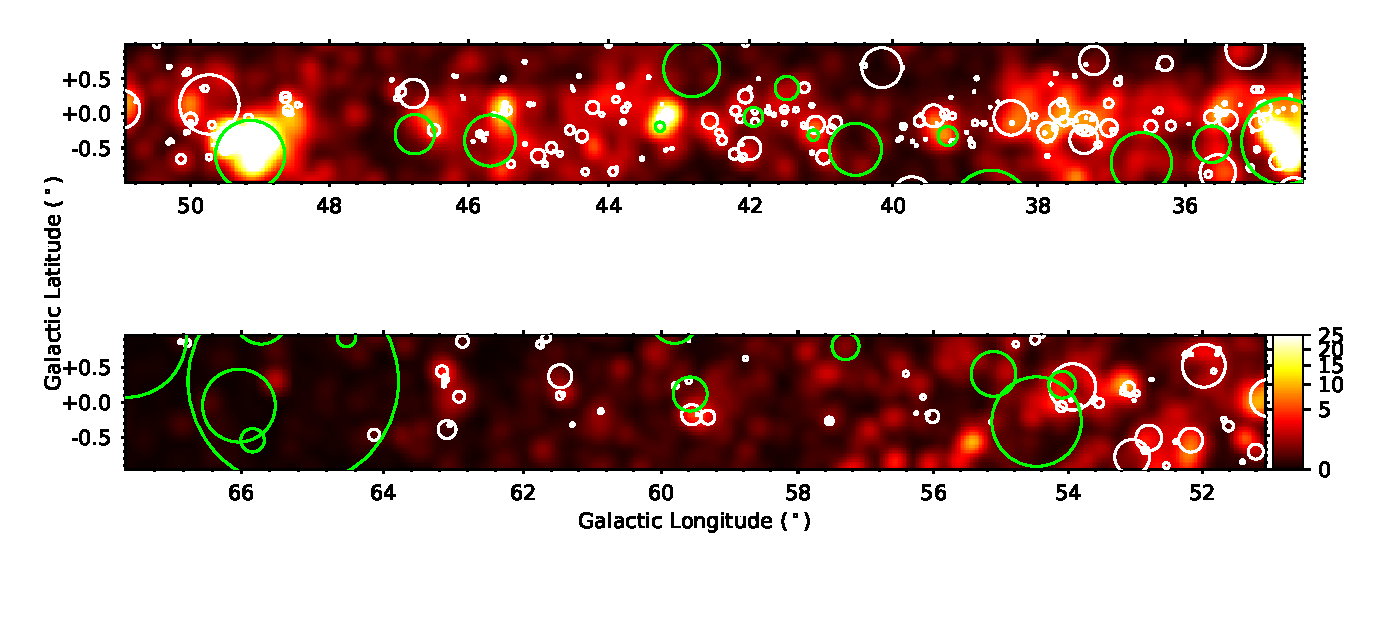
\includegraphics[width = 7in]{temperature_thermal_map.eps}
\caption{Free-Free continuum intensity. $T_{C}$ is calculated following Equation \ref{equ_temp}, using the SIGGMA H-RRL 0$^{th}$ moment map (integrated over $-20 - 120$\kms) and assuming $T_e = 8000 K$. The unit for the map is in Kelvin. The white circles are ``known'' HII regions from the WISE catalog and the blue circles are SNRs from the Green catalog (see Section \ref{sec_snr}). The bright spots between $l=55\degr-57\degr$ are likely artificial effects due to missing data (see Figure \ref{fig_skycover}).}
\label{fig_gal_free}
\end{figure}
\begin{figure}[bhpt]
\centering
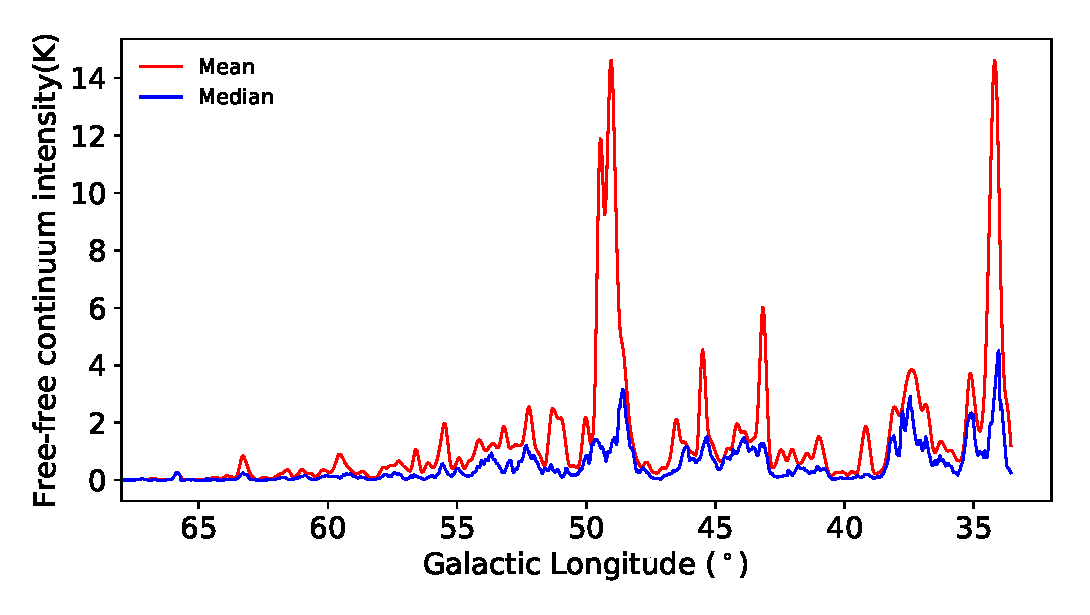
\includegraphics[width = 6in]{temperature_thermal_plot.eps}
\caption{Free-Free Continuum Intensity as a function of Galactic longitude. The red line is the mean temperature over $|b|\le 1\degr$. The blue line is the median value over the same range.}
\label{fig_gal_plot}
\end{figure}

\section{Carbon RRL emission regions} \label{sec_crrl}
C-RRLs are offset by $\sim-150$\kms\ from H-RRLs for the same principle quantum numbers.
SIGGMA detects H-RRL emission from the velocity range of $\sim -50$ to $150$\kms\ (cf.~Figure~\ref{lv_map}).
To identify C-RRL emission regions, we modify the SIGGMA datacubes by shifting the velocity to center at the C-RRL rest frequency.
We create C-RRL moment maps from the shifted cubes by integrating over the same velocity range as we did for H-RRLs.
Table\,\ref{tab_crrl} contains information about the C-RRL regions. % EXPLAIN COLUMNS OF TABLE, SAME FOR OTHER TABLES
In this table, we list the region name,
the Galactic coordinate centroid, the angular size, the WISE catalog \hii\ region that is spatially coincident, the integrated C-RRL intensity, the H- to C-RRL integrated intensity ratio, and a qualitative assessment of the C-RRL data quality (A=highest quality, C=low quality).
Since the line widths for C-RRLs are $\lesssim$ 10\kms, the SIGGMA velocity resolution likely broadens the C-RRLs and decreases their intensities.
Instead of fitting Gaussian profiles, therefore compute the integrated intensity.

Carbon RRL emission is thought to arise from PDRs, and can be used to investigate PDR properties \citep[][etc.]{Pankonin1977,Natta1994,Roshi2007}.
Polycyclic aromatic hydrocarbon (PAH) molecules in PDRs emit at 8.0$\um$ \citep{Watson2008,Watson2009}, and we therefore expect a good agreement between C-RRL and 8.0$\um$ emission.
We compare the C-RRL emission distribution with the {\it Spitzer} 8.0\,\micron\ infrared data from the Galactic Legacy Infrared Midplane Survey Extraordinaire (GLIMPSE) Legacy Program \citep{Benjamin2003,Churchwell2009}.
%Since the dust within the \hii\ regions is heated by the central star and re-emits in mid-infrared (MIR), there is a strong correlation between \hii\ regions and their MIR images \citep{Wood1989,Kurtz1994,Anderson2011}.
Figure\,\ref{fig_crrl-g342} gives an example of those C-RRL regions.
We also include in this figure 24$\um$ {\it Spitzer} data from the MIPSGAL survey \citep{Carey2009, Gutermuth2015}.
This figure shows the spectral grid overlying the integrated C-RRL intensity map, and contours of the integrated C-RRL emission over the {\it Spitzer} three-color map (red: 24\,$\um$, green: 8\,$\um$, blue: 4.5\,$\um$).
For the source G34.2$+$0.2, the integrated C-RRL emission peaks on the corresponding \hii\ region as defined by the infrared emission.
%We also show the integrated H-RRL emission.
We find an extended C-RRL structure to the north, but the 8.0$\um$ emission is weak there, making the PDR origin of this emission doubtful.
More figures of detected C-RRL regions are given in Appendix\,\ref{appe:crrl}.
For G34.7$-$0.6 and G35.1$-$0.7 (see Figures \ref{fig_crrl-g347} and \ref{fig_crrl-g351}), we see the C-RRL emission regions are offset relative to the \hii\ regions.
The background of spectral grid maps of some C-RRL regions show that the C-RRL emission regions have an annular structure, with stronger emission regions surrounding weaker emission regions (see Figures \ref{fig_crrl-g389}, \ref{fig_crrl-g536}, \ref{fig_crrl-g609}, \ref{fig_crrl-g614}, and \ref{fig_crrl-g631} in Appendix\,\ref{appe:crrl}).
This may imply the emission feature from PDRs, although the morphologies do not agree that seen at 8.0\,\micron.

\begin{table}[htbp]
\caption{C-RRL emission regions}\label{tab_crrl}
\begin{threeparttable}
\begin{tabular*}{\textwidth}{cccclclc}
\hline
\hline
Name& $l$& $b$&Radius&\hii\ Region&$\int I_{CRRL}dV$& C/H$^a$& Quality$^b$\\
&deg.&deg.&deg.&&Jy\kms&&\\
\hline
G34.2$+$0.2& 34.24& $+$0.15& 0.05&G034.256$+$00.136 (NRAO584) &0.07& 0.03 & B\\
G34.7$-$0.6& 34.73& $-$0.58& 0.05&G034.757$-$00.669           &0.15& 0.03 & C\\
G35.1$-$0.7& 35.12& $-$0.71& 0.03&G035.126$-$00.755           &0.12& 0.38 & B\\
G38.9$-$0.4& 38.93& $-$0.42& 0.05&G038.926$-$00.389           &0.03& \nodata$^c$& B\\
G43.2$-$0.0& 43.16& $-$0.00& 0.05&G043.170$-$00.004 (W49A)    &0.58& 0.08 & A\\
G45.5$+$0.0& 45.46& $+$0.07& 0.05&G045.453$+$00.044 (K47)     &0.10& 0.08 & B\\
G49.5$-$0.4& 49.49& $-$0.40& 0.05&G049.484$-$00.391 (W51A)    &0.83& 0.07 & A\\
G53.6$+$0.0& 53.57& $+$0.02& 0.03&G053.541$-$00.011           &0.05& 0.50 & B\\
G60.9$-$0.1& 60.88& $-$0.11& 0.05&G060.881$-$00.135 (S87)     &0.03& 0.30 & A\\
G61.4$+$0.1& 61.44& $+$0.13& 0.05&G061.473$+$00.094 (S88)     &0.24& 0.24 & B\\
G63.1$+$0.4& 63.14& $+$0.38& 0.05&G063.164$+$00.449 (S90)     &0.10& 0.06 & C\\
\hline
\end{tabular*}
\begin{tablenotes}
      \small
      \item a. Integrated intensity ratio of H-RRL and C-RRLs.
      \item b. Qualitative metric of data quality (A=high quality, C=low quality)
      \item c. There is no valid H-RRL detection since a H-RRL signal is in the off position.
\end{tablenotes}
\end{threeparttable}
\end{table}

\begin{figure}[htbp]
\centering
\subfloat[SIGGMA spectral grid]{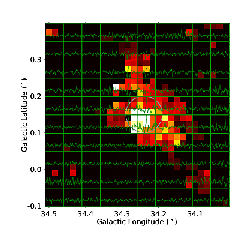
\includegraphics[width = 3.3in]{crrl_eps/G34.2+0.2_ca_spec.eps}}
\subfloat[Infrared color map  ]{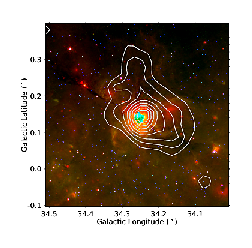
\includegraphics[width = 3.3in]{crrl_eps/G34.2+0.2_rgb_contour.eps}}\\
\subfloat[SIGGMA spectral grid]{\includegraphics[width = 3.3in]{crrl_eps/G34.2+0.2_ha_spec.eps}}
\subfloat[Infrared color map  ]{\includegraphics[width = 3.3in]{crrl_eps/G34.2+0.2_ha_rgb_contour.eps}}\\ 
\caption{The C-RRL region G34.2+0.2.
          (a) The C-RRL grid with velocity from $-50$ to $150$\kms.
	  The background is the integrated C-RRL intensity over 30 to 70\kms.
	  (b) The infrared RGB map (r: 24\,$\um$, g: 8\,$\um$, b: 4.5\,$\um$) overlaid with integrated C-RRL contours.
	  The contour levels are 2, 4, 6, 8, 10, 12, 14, 16 mJy\,beam$^{-1}$\kms.
	  (c) The H-RRL grid with velocity from $-50$ to $150$\kms.
	  The background is the integrated C-RRL intensity over 0 to 100\kms.
	  (d) The infrared RGB map (r: 24\,$\um$, g: 8\,$\um$, b: 4.5\,$\um$) overlaid by integrated H-RRL contours.
	  The levels are 0.2, 0.4, 0.6, 0.8, 1, 1.2, 1.4, 1.6 Jy\,beam$^{-1}$\kms.
	  }
\label{fig_crrl-g342}
\end{figure}

\section{RRLs from Galactic supernova remnants} \label{sec_snr}

SNRs are strong non-thermal radio sources.
Early studies have however reported RRL detections toward Galactic SNRs \citep{Downes1974,Pankonin1976}.
These authors concluded that the RRLs likely originated in low-brightness \hii\ regions along the line of sight.
\cite{Onic2012} investigated the possibility of significant production of thermal bremsstrahlung radiation from Galactic SNRs, from which the radio continuum has a flattening at higher frequencies and thermal absorption at lower frequencies. They suggested that for the source 3C396 there could be a thermal contamination.
However, \citep{Cruciani2016}, with their multi-frequency radio continuum and polarization observations, confirmed that 3C 396 emission is dominated by synchrotron emission.
We examine the SIGGMA RRL emission in the direction of Galactic SNRs.
The morphology provided by the RRL maps may also help to infer whether the RRLs come from SNRs or not.

\cite{Green2014} updated their comprehensive Galactic SNR catalog (hereafter the Green catalog).
The SIGGMA survey contains 32 SNRs that are listed in this catalog.
Some SNRs with large radi are faint and some are overlapped with one or more \hii\ regions; these are not ideal candidates for SIGGMA RRL detections.
By examining the continuum emission at 1.4\,GHz from the VLA Galactic Plane Survey \citep[VGPS,][]{Stil2006} and the location of nearby \hii\ regions, we extract the spectra of 14 SNRs (see Table\,\ref{tab_snr}).
In this table, we list the names of the SNRs, the Galactic coordinate of the central region and its radius,
 the integrated intensity of H-RRL emission averaged over the region,
 the LSR velocity of the peak H-RRL emission, and the calculated near and far kinematic distances using the \citet{Reid2014} rotation curve.  For all regions, one of the two kinematic distances agrees well with the distance from the literature, indicating that the H-RRLs do indeed come from the SNRs themselves.

The line widths of the detected H-RRLs from SNRs are broad. 
This implies that the temperature and/or turbulent motions of the plasmas are higher than that of \hii\ regions.
However, the broad line width makes the spectrum more likely to be affected by baseline fitting.
The high continuum intensity of the SNRs may also introduce uncertainties due to baseline issues. 
Uncertainties in derived RRL parameters from SNRs are therefore larger than those of \hii\ regions.
In this case, the formal fitting errors of the line profiles are relatively small compared to the larger uncertainties due to baseline structure; we do not attempt to quantify the parameter uncertainties in Table\,\ref{tab_snr}.
Most detected SNRs show a similar broad line profile.
The agreement between SNR profiles implies that despite the baseline uncertainties, these detections are real.

Figure\,\ref{fig_snr-g347} shows the SIGGMA RRL detection toward SNR G34.7$-$0.4 with the SIGGMA spectral grid overlaid on the integrated H-RRL intensity map (left) and VGPS continuum with integrated RRL contours overlaid (right).
The RRL emission intensity is correlated with the continuum intensity, indicating significant thermal continuum emission.
The spectral profiles vary over the source.
Within the central region, the lines are broad with strongly varying peak intensities.
At the northeast and southeast edge there are \hii\ regions (blue circles in Figure\,\ref{fig_snr-g347} (b)), the spectra are combinations of broad and narrow Gaussian features.  The excellent agreement between H-RRL and continuum morphologies again indicates that the H-RRLs arise from the SNR and not \hii\ regions along the line of sight.
Figures for other SNRs listed in Table\,\ref{tab_snr} are given in Appendix\,\ref{appe:snr}.

\begin{table}[htbp]
\renewcommand{\arraystretch}{0.8}
\caption{ H-RRL detections from SNRs}\label{tab_snr}
\begin{threeparttable}
\begin{tabular*}{\textwidth}{l@{\extracolsep{\fill}}*{12}{c}}
\hline
\hline
GName$^a$&Other Name& $l$& $b$& Radius&V$_{LSR}$&FWHM&D$_{N}$&D$_{F}$&D& Quality$^c$\\
&& deg.&deg.& deg.& \kms&\kms&kpc&kpc&kpc&\\
\hline
G33.6$+$0.1&Kes 79 & 33.67& $+$0.03& 0.11 &106.3&26.1 &6.4 &7.5  &7.1$^{[1]}$     &C\\ 
G34.7$-$0.4&W44    & 34.67& $-$0.42& 0.32 &47.7 &114.3& 2.9   &10.8 &2.9$^{[2]}$     &B\\
           &       &      &        &      &49.4 &11.6 &3.0 &10.7 &&\\
           &       &      &        &      &138.0&80.0 & 6.8   & 6.8    &&\\
G35.6$-$0.4&       & 35.60& $-$0.43& 0.13 &53.7 &23.5 &3.2 &10.3 &3.6$^{[3]}$     &A\\ 
G36.6$-$0.7&       & 36.59& $-$0.69& 0.28 &40.6 &64.4 &2.5    &10.8     &\nodata         &B\\
           &       &      &        &      &57.5 &20.2 & 3.4   & 9.9    &&\\
           &       &      &        &      &146.0&71.5 &6.7 &6.7 &&\\
G39.2$-$0.3&3C 396 & 39.23& $-$0.32& 0.08 &12.8 &34.0 &0.8    &9.2     &$\leq11.3^{[4]}$&A\\ 
           &       &      &        &      &61.2 &24.5 &3.7 &9.2  &&\\
G40.5$-$0.5&       & 40.51& $-$0.51& 0.23 &45.3 &36.1 &2.8 &9.8 &\nodata         &C\\
G41.1$-$0.3&3C 397 & 41.12& $-$0.31& 0.05 &62.1 &24.5 &3.8 &8.7 &10.3$^{[5]}$    &A\\ 
G41.5$+$0.4&       & 41.46& $+$0.39& 0.12 &19.2 &18.2 &1.3 &11.2 &10.3$^{[6]}$    &A\\ 
G43.3$-$0.2&W49B   & 43.27& $-$0.19& 0.07 &9.1  &42.5 &0.6 &11.5     &7.5$^{[1]}$,10$^{[7]}$      &A\\ 
           &       &      &        &      &62.7 &24.7 &4.1 &8.0  &&\\
G45.7$-$0.4&       & 45.56& $-$0.35& 0.21 &65.1 &18.6 &4.8 &6.8  &\nodata         &B\\
           &       &      &        &      &86.5 &100.4 &5.8    &5.8     &&\\
G46.8$-$0.3&HC 30  & 46.77& $-$0.27& 0.16 &60.2 &25.3 &4.4 &7.0  &6.4$^{[1]}$     &C\\
G49.2$-$0.7&W51C   & 49.14& $-$0.61& 0.22 &62.3 &41.2 &5.4 &5.4  &6$^{[1]}$       &A\\
           &       &      &        &      &122.8&51.8  &5.4    &5.4     &&\\
G54.4$-$0.3&HC 40  & 54.47& $-$0.29& 0.38 &43.6 &15.5 &4.1 &5.6  &3.3$^{[1]}$,6.6$^{[8]}$     &B\\
G57.2$+$0.8&4C21.53& 57.24& $+$0.82& 0.10 &106.1&39.8 &4.5 &4.5  &\nodata         &B\\ 
\hline
\end{tabular*}
\begin{tablenotes}
      \small
      \item a. Names are defined using the Galactic coordinates given by \cite{Green2014}.
      \item b. Integrated intensity over the velocity range of 0 to 150\kms.
      \item c. Qualitative metric of data quality (A=high quality, C=low quality)
      \item REFERENCES: [1] \citet{Case1998};[2] \citet{Seta1998};[3] \citet{Zhu2013};[4] \citet{Caswell1975}; [5] \citet{Safi-Harb2005}; [6] \citet{Pavlovic2014}; [7] \citet{Zhu2014}; [8] \citet{Ranasinghe2017};
      \end{tablenotes}
\end{threeparttable}

\end{table}

\begin{figure}[htbp]
\centering
\subfloat[SIGGMA spectral grid]{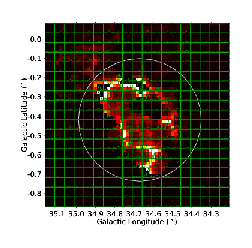
\includegraphics[width = 3.5in]{snr_eps/G34.7-0.4_ha_spec.eps}}
\subfloat[VGPS 1.4 GHz continuum map]{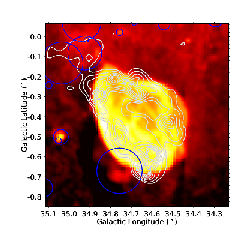
\includegraphics[width = 3.5in]{snr_eps/G34.7-0.4_vgps_contour.eps}}\\
\caption{The H-RRL emission from SNR: G34.7-0.4.
          (a) The SIGGMA spectral grid with the velocity range from $-300$ to $300$\kms.
	  The background is the 0$^{th}$ moment C-RRL map over $0$ to $150$\kms.
	  The white circle is the central region of the SNR.
	  (b) The VGPS 1.4 GHz continuum map overlaid by integrated RRL contour.
	  The levels are 0.5, 1, 2, 3, 4, 5, 6, 7 Jy\,beam$^{-1}$\kms.
	  The blue circles are location of \hii\ regions.
	  }
\label{fig_snr-g347}
\end{figure}

\section{Individual RRL emission regions}\label{sec_indi}

SIGGMA maps of \hii\ regions can reveal information not apparent in single-pointing RRL observations.  To illustrate this, we present the RRL analysis of two large star-forming regions, W49 and W51.

\subsection{W49}
The W49 star-forming complex can be separated into sub-regions W49A and W49B.
W49A is among the most luminous star formation complexes in the Galaxy and is located at a distance of 11.11$^{+0.79}_{-0.69}$\,\kpc\ reported by \citet{Zhang2013} from trigonometric parallax measurements of H$_{2}$O masers.
W49B is a SNR whose centroid is $\sim$ 12$\arcmin$ from that of W49A \citep{Lacey2001}.
In the W49A region, there are compact radio sources with RRL emission that are embedded in diffuse ionized gas \citep{Depree1997,Depree2003}.
Although W49A has many embedded ultra-compact \hii\ regions, due to beam dilution the RRL emission observed by SIGGMA likely arises mostly from diffuse gas.
Also, at L-band, compact \hii\ regions may be optically thick and therefore may not contribute as much to the observed RRL emission as they would at higher frequencies.

Figure~\ref{w49_spec_map} (a) shows the SIGGMA RRL spectral grid for the W49 complex.
RRL emission is detected over the entire region.
In addition to the known velocity of W49A, $\sim$10\kms, there is a second velocity component around $\sim$60\kms\ found toward both W49A and W49B (Figure \ref{w49_spec_map} (b)).
This 60\kms\ component has been detected previously.
\citet{Downes1974} reported the RRL detection in the direction of W49B with a LSR velocity of 65\kms.
\citet{Pankonin1975} also detected RRL towards W49B at LSR velocity of 60\kms.
\citet{Anantharamaiah1986} detected a RRL velocity of 63\kms\ toward W49A (G43.2-0.1).
Figure \ref{w49_spec_map} panels (c) and (d) show the RRL intensity contours of the two velocity components overlaid on top of VGPS continuum data.
The 60\kms\ RRL component is also found toward W49A, although some of its intensity could arise from the line wing of 10\kms\ component.
Both of the velocity distributions peak at the two sources, although the W49B peaks are offset towards the Galactic east.
The spatial mismatch may imply that the thermal RRL emission region is different from that of the non-thermal synchrotron emission.

The fact that there are two velocity components for the region is confusing. The kinematic distance for W49A from the 10\kms\ component agrees with the known distance for this region, so we can assume that the 10\kms\ component comes from gas 11.4\kpc\ distant. It therefore is possible that the 60\kms\ component comes from W49B, and its distance is quite different from that of W49A.
Previous \hi\ absorption studies suggested W49B at a distance of $\sim$8.0\kpc\ \citep{Moffett1994} or $\sim$11.4\kpc\ \citep{Brogan2001}.
Recent work by \citet{Zhu2014} assigned W49B a velocity of 40\kms\ at distance about $\sim$10\kpc.

To determine if the 60\kms\ component comes from W49B, we analyze VGPS HI data in its direction (Figure \ref{w49_hi}).
Along this sight line there is near and far gas with velocities from 0$-$70\kms.
It seems that essentially all velocities where W49A shows absorption have corresponding absorption for W49B, except for near 10\kms\ and 60\kms. 
So the 10\kms\ RRL in the direction of W49B seems not likely from W49B.
While the case of 60\kms\ component is complicated and needs further study.

\begin{figure}[htbp]
\centering
\subfloat[Integrated RRL intensity map overlaid with spectral lines.]{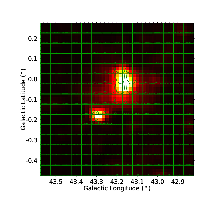
\includegraphics[width = 3.3in]{w49_spec_map.eps}}
\subfloat[H-RRL spectra of W49A and W49B]{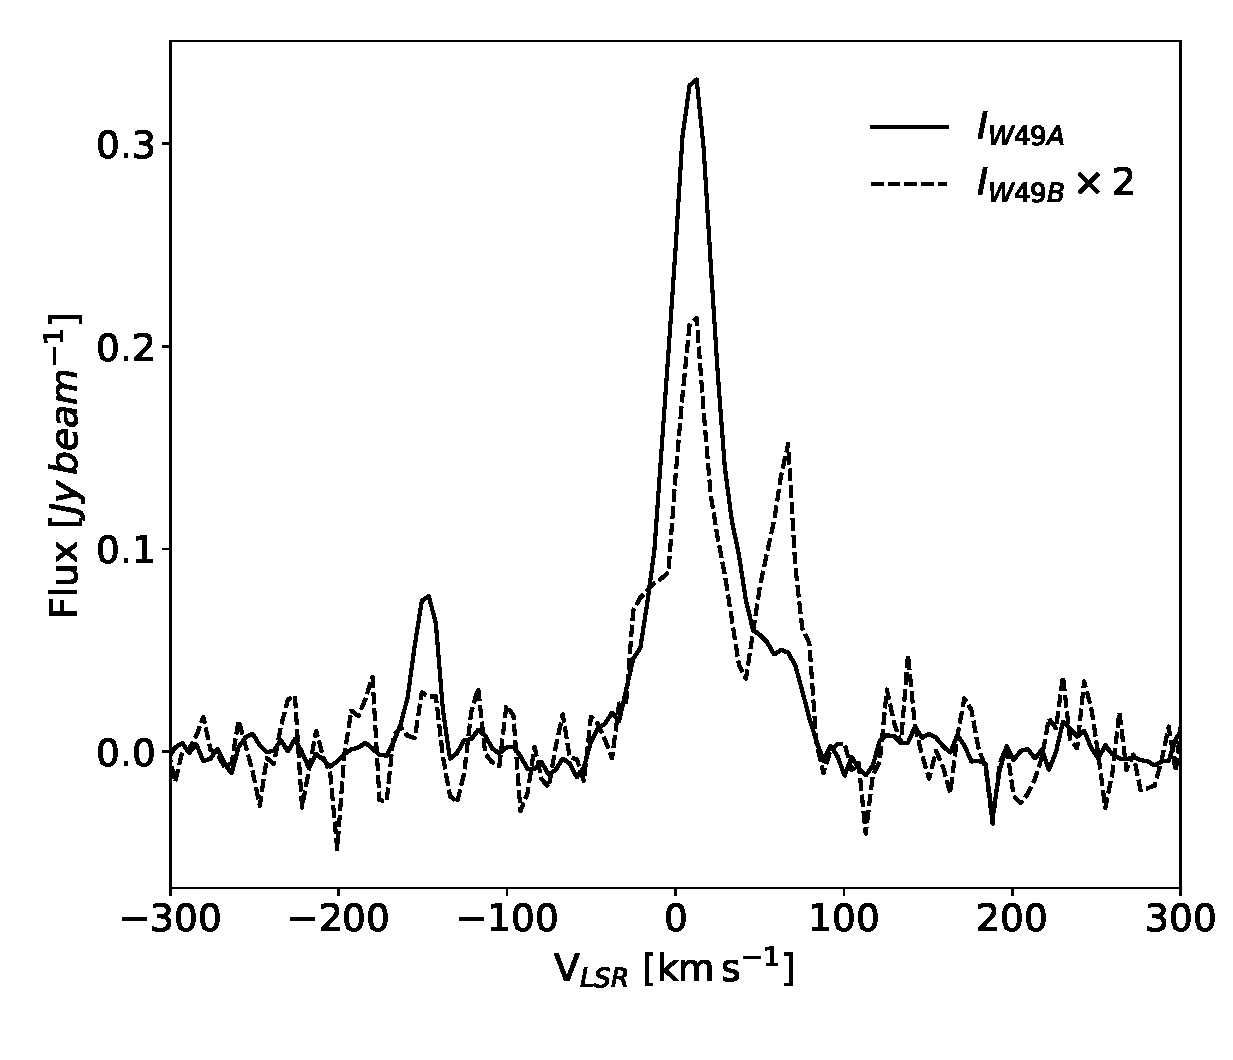
\includegraphics[width = 3.3in]{w49_spec_plot.eps}}\\
\subfloat[The 10\kms\ velocity component]{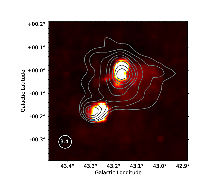
\includegraphics[width = 3.3in]{w49_vgps_siggma_v1.eps}}
\subfloat[The 60\kms\ velocity component]{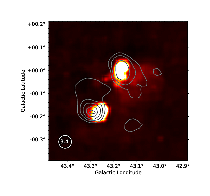
\includegraphics[width = 3.3in]{w49_vgps_siggma_v2.eps}}\\
\caption{Integrated RRL intensity maps of the W49 region. (a) The RRL spectral grid. The background image is of RRL integrated intensity integrated over the velocity range from 0 to 70\kms.
(b) shows the spectral plots of W49A and W49B. The line intensity of W49B is enlarged by factor of 2 so that its detail can be seen.
(c) and (d) are the SIGGMA integrated intensity RRL contours overlaid on VGPS 1.4\ghz\ continuum data.  The SIGGMA data were integrated over $0-20$\kms\ (panel c) and $50-70$\kms\ (panel d).
The SIGGMA contour levels are at values of 0.05, 0.1, 0.2, 0.4, 0.6, 1.0, 1.4, and 1.8 Jy\,beam$^{-1}$\kms\ for (c) and 0.05, 0.1, 0.2, 0.4, and 0.6 Jy\,beam$^{-1}$\kms\ for (d).
}\label{w49_spec_map}
\end{figure}

\begin{figure}[htbp]
\centering
\plotone{w49_hi_plot.eps}
\caption{The \hi\ absorption spectra towards W49A and W49B. For the reason of comparison, we present two spectrum for each source and add 0.5 to separate the W49A2 and W49B2.  }\label{w49_hi}
\end{figure}
\subsection{W51}
The W51 region is another enormous first-quadrant star formation complex.
It is located near the tangent point in the Sagittarius Arm at a distance of 5.41$^{+0.31}_{-0.28}$\kpc\ measured by means of trigonometric parallax \citep{Sato2010}, and is grouped into three regions, W51A, W51B, and W51C.
W51A and W51B are massive star-forming regions, whereas W51C is a SNR \citep{Subrahmanyan1995}.
Pointed RRL observations toward W51 have been carried out \citep{Pankonin1979,Anderson2011}, showing that it can be decomposed into multiple discrete \hii\ regions.

Similarly to W49, much of the SIGGMA RRL emission from W51 is likely due to diffuse gas rather than from compact \hii\ regions.
Figure \ref{w51_map} shows the comparison of the integrated RRL contours from SIGGMA, 1.4 GHz continuum map in blue from the VGPS, and the infrared map from {\it Spitzer} (8$\um$ in green and 24 $\um$ in red).
The infrared emission indicates the emission from \hii\ regions.
The contour corresponding with the ``known'' \hii\ region (the red circle in Figure \ref{w51_map}) shows the capability of SIGGMA for detecting weak RRL emission.
It is indicated that the SIGGMA RRL map is sensitive to not only the discrete \hii\ regions but also the diffuse gases in between.
The RRL contours match with the strong infrared emission and also shows some RRL emitting regions where the infrared emission is not obvious.
To the west of W51B in Figure \ref{w51_map} (around G48.5$-$0.2), RRLs are detected from diffuse ionized gas, which shows a bubble-like feature in the infrared.
The lack of infrared emission at locations of strong RRL emission implies that the RRL emission may be due to leaking photons from \hii\ regions.

Figure \ref{fig_crrl-g494} in Appendix \ref{appe:crrl} and Figure \ref{fig_snr-g492} in Appendix \ref {appe:snr} give the spectral grid maps and integrates RRL contours of the W51 region.
As we saw for other SNRs, there is strong RRL emission toward W51C, which is bright in 1.4 GHz continuum but weak in the infrared.
The LSR velocities of SIGGMA-detected RRLs from W51A, W51B, and W51C are 62.8\kms, 66.4\kms, and 62.3\kms, indicating that they are physically related.
This agrees well with the comprehensive studies in the literature \citep{Mufson1979, Mehringer1994, Brogan2013}.
\citet{Koo1997a, Koo1997b} studied the interaction between W51C and a nearby molecular cloud.
From the interface between the SNR and the surrounding molecular cloud, they found high velocity emission line components of CO and HCO$^{+}$ around 100\kms, as well as high velocity \hi\ gas with similar V$_{LSR}$.
Coincidentally, there is also an second velocity RRL component at 122.8\kms\ towards W51C detected by SIGGMA, indicating that RRLs could originate from the shocked gas between SNR and molecular gas.

\begin{figure}[htbp]
\centering
\plotone{w51_rgb_siggma.eps}
\caption{Three-color map of W51 
with {\it Spitzer} 24 $\um$ data in red,  {\it Spitzer} 8 $\um$ data in green, and VGPS 1.4\ghz\ continuum data in blue. 
SIGGMA H-RRL contours are overlaid at levels of 0.05, 0.15, 0.3, 0.45, 0.6, 0.9, 1.2, 1.5, 1.8, and 2.1 Jy\,beam$^{-1}$\kms. The red circle shows the location and radius of a ``known'' \hii\ region from the WISE catalog, illustrating SIGGMA's ability to detect faint RRL emission. The blue circle shows the location of the SNR W51C with the radius from the Green catalog.}\label{w51_map}
\end{figure}

\section{Summary} \label{sec_summ}
SIGGMA is the most sensitive large-scale RRL survey extent.
The average rms level of the SIGGMA spectra is $\sim 0.65$ mJy.
The sky coverage of the released data is $l=32\degr - 70\degr$, $|b|\le 1.5\degr$.

We have produced RRL maps from the SIGGMA data observed with a FWHM of 3.4$\arcmin$ and a spectral resolution of 5.1\kms. 
Both discrete \hii\ regions and diffuse ionized gas can be seen in the maps.
By matching with the WISE catalog, we provide RRL profile parameters of the known and candidate \hii\ regions.
We have also examined carbon RRL emission along the inner Galactic plane.
Although C-RRLs are weak and the SIGGMA spectra have baseline ripples, we did detect C-RRLs.
RRL emission from SNRs is another topic allowed by the SIGGMA data.
We have extract all the spectra toward SNRs in the SIGGMA survey area.
More than half of them show emission line features, indicating that RRL emission may be a useful way to determine SNR distances.

To illustrate the utility of SIGGMA data toward star formation complexes, we discussed results toward the two bright star-forming complexes, W49 and W51.
Our analysis of the SNR W49B data indicate that the 10\kms\ RRL component is unlikely associated with the SNR and the origin of the 60\kms\ is not clear.
RRLs from the SNR W51C are with similar LSR velocities to W51A and W51B.
Also a high velocity RRL component toward W51C is detected, which matches with the high velocity component of nearby molecular cloud and \hi\ gases.

The survey data are available online in standard fits files format.\footnote{WE NEED TO DISCUSS WHERE TO PUT AND WHAT TO PUT?}

\acknowledgments
\newpage
\appendix

\section{Catalogues of detected \hii\ regions}\label{appe:cata}
\begin{ThreePartTable}
\begin{longtable}{lccccccc}
\caption{Catalog of 319 RRL detections towards 244 ``known'' HII regions from the WISE catalog\label{tab_HII_known}} \\
\hline
\hline
Name & $l$ & $b$ & Peak& V$_{LSR}$& FWHM& RMS& $S/N$\\
&$^\circ$&$^\circ$&mJy\,beam$^{-1}$&km\,s$^{-1}$&km\,s$^{-1}$&mJy\,beam$^{-1}$& \\
\hline
\endfirsthead
\caption{continued \ldots}\\
\hline
\hline
Name & $l$ & $b$ & Peak& V$_{LSR}$& FWHM& RMS& $S/N$\\
&$^\circ$&$^\circ$&mJy\,beam$^{-1}$&km\,s$^{-1}$&km\,s$^{-1}$&mJy\,beam$^{-1}$& \\
\hline
\endhead
\hline
\endfoot
\hline
\endlastfoot
G032.800$+$00.190     &32.800&	$+$0.190	&9.16	$\pm$ 1.01	&14.9	$\pm$ 1.2	&22.1	$\pm$ 2.8	&1.65	&8.9 \\ 
G032.823$+$00.072$^a$ &32.824&	$+$0.072	&30.40	$\pm$ 2.89	&106.7	$\pm$ 1.2	&25.3	$\pm$ 2.8	&2.76	&19.0\\
G032.835$+$00.017     &32.835&	$+$0.017	&191.52	$\pm$ 22.13	&109.8	$\pm$ 1.8	&33.3	$\pm$ 4.8	&28.51	&13.2\\
G032.982$-$00.338     &32.983&	$-$0.338	&17.08	$\pm$ 2.16	&50.8	$\pm$ 1.2	&20.6	$\pm$ 3.3	&2.56	&10.3\\
G033.051$-$00.078     &33.051&	$-$0.078	&26.21	$\pm$ 1.76	&103.9	$\pm$ 0.9	&28.0	$\pm$ 2.3	&0.77	&61.2\\
G033.080$+$00.073     &33.080&	$+$0.073	&11.65	$\pm$ 0.97	&102.2	$\pm$ 1.1	&27.8	$\pm$ 2.7	&1.22	&17.3\\
G033.142$-$00.088$^a$ &33.142&	$-$0.087	&20.93	$\pm$ 1.52	&103.2	$\pm$ 0.9	&26.4	$\pm$ 2.2	&1.19	&30.9\\
G033.176$-$00.016     &33.176&	$-$0.015	&27.82	$\pm$ 2.09	&105.1	$\pm$ 1.0	&26.2	$\pm$ 2.3	&1.63	&29.9\\
G033.205$-$00.013     &33.205&	$-$0.012	&14.64	$\pm$ 2.52	&106.5	$\pm$ 1.1	&13.1	$\pm$ 2.6	&2.46	&7.4\\
G033.263$+$00.066     &33.263&	$+$0.067	&11.51	$\pm$ 1.06	&111.3	$\pm$ 1.9	&42.2	$\pm$ 4.5	&1.40	&18.2\\
G033.419$-$00.005     &33.419&	$-$0.004	&14.86	$\pm$ 1.71	&100.7	$\pm$ 2.0	&35.6	$\pm$ 4.7	&2.45	&12.3\\
G033.809$-$00.186$^a$ &33.810&	$-$0.185	&25.78	$\pm$ 2.91	&50.9	$\pm$ 1.0	&18.7	$\pm$ 2.4	&3.67	&10.4\\
                      &33.810&	$-$0.185	&14.74	$\pm$ 2.42	&102.8	$\pm$ 2.2	&27.1	$\pm$ 5.1	&3.67	&7.1\\
G033.809$-$00.190$^a$ &33.809&	$-$0.190	&25.78	$\pm$ 2.91	&50.9	$\pm$ 1.0	&18.7	$\pm$ 2.4	&3.67	&10.4\\
                      &33.809&	$-$0.190	&14.74	$\pm$ 2.42	&102.8	$\pm$ 2.2	&27.1	$\pm$ 5.1	&3.67	&7.1\\
G033.882$+$00.057     &33.882&	$+$0.057	&4.98	$\pm$ 0.41	&59.3	$\pm$ 3.2	&77.2	$\pm$ 7.4	&1.23	&12.1\\
G033.914$+$00.107     &33.915&	$+$0.108	&7.72	$\pm$ 0.67	&103.8	$\pm$ 2.5	&57.3	$\pm$ 5.8	&1.09	&18.4\\
G033.941$-$00.039     &33.942&	$-$0.039	&21.87	$\pm$ 1.34	&62.1	$\pm$ 0.6	&19.3	$\pm$ 1.4	&2.04	&16.1\\
G033.987$-$00.012$^a$ &33.988&	$-$0.011	&14.47	$\pm$ 0.50	&56.4	$\pm$ 0.7	&37.9	$\pm$ 1.5	&1.07	&28.4\\
G033.991$-$00.005$^a$ &33.991&	$-$0.004	&14.47	$\pm$ 0.50	&56.4	$\pm$ 0.7	&37.9	$\pm$ 1.5	&1.07	&28.4\\
G034.026$-$00.058     &34.026&	$-$0.058	&22.76	$\pm$ 2.53	&59.1	$\pm$ 1.0	&15.0	$\pm$ 1.5	&0.90	&33.3\\
                      &34.026&	$-$0.058	&11.51	$\pm$ 1.43	&42.5	$\pm$ 2.7	&19.5	$\pm$ 4.5	&0.90	&19.2\\
                      &34.026&	$-$0.058	&5.02	$\pm$ 0.40	&96.5	$\pm$ 5.9	&83.1	$\pm$ 12.2	&0.90	&17.3\\
G034.041$+$00.052$^a$ &34.041&	$+$0.053	&7.45	$\pm$ 0.43	&53.1	$\pm$ 1.9	&36.4	$\pm$ 4.3	&0.86	&17.8\\
G034.045$+$00.053$^a$ &34.046&	$+$0.053	&7.45	$\pm$ 0.43	&53.1	$\pm$ 1.9	&36.4	$\pm$ 4.3	&0.86	&17.8\\
G034.104$-$00.046     &34.105&	$-$0.046	&32.30	$\pm$ 2.54	&49.9	$\pm$ 0.9	&36.5	$\pm$ 3.0	&1.97	&33.9\\
G034.158$+$00.147     &34.158&	$+$0.148	&15.69	$\pm$ 1.87	&61.7	$\pm$ 0.6	&17.2	$\pm$ 1.9	&0.94	&23.6\\
                      &34.158&	$+$0.148	&11.11	$\pm$ 1.90	&49.7	$\pm$ 2.7	&43.6	$\pm$ 5.1	&0.94	&26.6\\
G034.256$+$00.136     &34.256&	$+$0.136	&151.57	$\pm$ 12.16	&54.9	$\pm$ 1.0	&36.9	$\pm$ 2.9	&6.66	&47.2\\
                      &34.256&	$+$0.136	&44.35	$\pm$ 4.21	&114.9	$\pm$ 8.6	&86.4	$\pm$ 17.9	&6.66	&21.2\\
G034.333$+$00.212     &34.333&	$+$0.213	&45.52	$\pm$ 2.47	&66.8	$\pm$ 0.5	&19.0	$\pm$ 1.3	&2.15	&31.5\\
G034.404$+$00.227     &34.404&	$+$0.228	&36.35	$\pm$ 1.30	&64.1	$\pm$ 0.3	&17.4	$\pm$ 0.7	&1.88	&27.6\\
G034.542$+$00.062     &34.542&	$+$0.062	&12.71	$\pm$ 5.74	&54.5	$\pm$ 5.0	&25.9	$\pm$ 6.1	&1.93	&11.5\\
G034.550$-$01.110     &34.550&	$-$1.110	&15.13	$\pm$ 0.89	&49.0	$\pm$ 0.5	&15.4	$\pm$ 1.1	&1.21	&16.7\\
G034.591$+$00.244     &34.591&	$+$0.244	&21.31	$\pm$ 1.81	&61.8	$\pm$ 0.7	&18.9	$\pm$ 2.0	&1.67	&18.9\\
                      &34.591&	$+$0.244	&6.95	$\pm$ 0.81	&114.3	$\pm$ 5.6	&73.9	$\pm$ 14.0	&1.67	&12.2\\
G034.686$+$00.068     &34.686&	$+$0.068	&15.52	$\pm$ 0.85	&58.6	$\pm$ 0.9	&34.6	$\pm$ 2.2	&1.73	&18.1\\
G034.756$+$00.022     &34.757&	$+$0.022	&22.29	$\pm$ 2.08	&53.2	$\pm$ 1.0	&21.8	$\pm$ 2.4	&3.34	&10.6\\
                      &34.757&	$+$0.022	&12.85	$\pm$ 2.52	&89.1	$\pm$ 1.4	&14.7	$\pm$ 3.4	&3.34	&5.0\\
G034.757$-$00.669     &34.757&	$-$0.668	&25.46	$\pm$ 2.24	&48.7	$\pm$ 0.4	&12.4	$\pm$ 1.0	&1.40	&21.9\\
                      &34.757&	$-$0.668	&10.30	$\pm$ 3.26	&27.6	$\pm$ 2.3	&28.5	$\pm$ 9.5	&1.40	&13.4\\
G034.916$-$00.016     &34.916&	$-$0.016	&25.62	$\pm$ 1.28	&48.8	$\pm$ 0.6	&31.3	$\pm$ 1.9	&1.60	&30.7\\
G034.924$-$00.082     &34.925&	$-$0.082	&35.20	$\pm$ 2.89	&49.2	$\pm$ 0.6	&19.0	$\pm$ 1.9	&1.85	&28.4\\
G034.940$+$00.073     &34.940&	$+$0.074	&21.63	$\pm$ 1.26	&52.1	$\pm$ 0.6	&25.2	$\pm$ 1.8	&1.61	&23.0\\
G034.997$+$00.330     &34.997&	$+$0.331	&12.34	$\pm$ 0.55	&59.3	$\pm$ 0.6	&26.5	$\pm$ 1.4	&0.98	&22.1\\
G035.040$-$00.500     &35.040&	$-$0.500	&32.33	$\pm$ 1.43	&48.8	$\pm$ 0.3	&15.7	$\pm$ 0.8	&1.97	&22.2\\
G035.051$-$00.520     &35.051&	$-$0.520	&12.06	$\pm$ 0.98	&46.5	$\pm$ 0.5	&13.7	$\pm$ 1.3	&1.25	&12.2\\
G035.063$+$00.330     &35.064&	$+$0.330	&10.35	$\pm$ 0.63	&56.4	$\pm$ 0.9	&18.2	$\pm$ 1.9	&0.91	&16.5\\
                      &35.064&	$+$0.330	&3.29	$\pm$ 0.61	&80.3	$\pm$ 2.8	&19.4	$\pm$ 6.5	&0.91	&5.4\\
G035.099$-$00.243     &35.099&	$-$0.243	&4.63	$\pm$ 0.39	&57.4	$\pm$ 4.0	&96.3	$\pm$ 9.5	&1.25	&12.4\\
G035.126$-$00.755     &35.126&	$-$0.754	&3.72	$\pm$ 0.54	&49.1	$\pm$ 1.9	&27.3	$\pm$ 4.6	&0.97	&6.8\\
G035.187$+$00.892     &35.187&	$+$0.893	&4.90	$\pm$ 0.24	&88.4	$\pm$ 0.5	&18.4	$\pm$ 1.1	&0.34	&20.9\\
G035.258$+$00.118     &35.259&	$+$0.119	&4.63	$\pm$ 0.33	&65.2	$\pm$ 2.7	&77.3	$\pm$ 6.4	&0.89	&15.6\\
G035.429$-$00.260     &35.430&	$-$0.260	&6.19	$\pm$ 0.60	&52.7	$\pm$ 1.5	&30.5	$\pm$ 3.4	&1.15	&10.1\\
G035.467$+$00.004     &35.467&	$+$0.004	&27.78	$\pm$ 0.74	&58.5	$\pm$ 0.4	&29.0	$\pm$ 0.9	&1.38	&37.0\\
G035.467$+$00.139     &35.468&	$+$0.139	&8.61	$\pm$ 0.56	&54.8	$\pm$ 1.2	&37.7	$\pm$ 2.9	&1.20	&15.1\\
G035.543$+$00.006     &35.543&	$+$0.007	&55.24	$\pm$ 0.98	&55.1	$\pm$ 0.2	&27.2	$\pm$ 0.6	&1.77	&55.6\\
G035.559$-$00.824     &35.560&	$-$0.823	&10.10	$\pm$ 0.58	&60.8	$\pm$ 1.1	&19.3	$\pm$ 1.7	&0.43	&35.5\\
                      &35.560&	$-$0.823	&3.02	$\pm$ 0.65	&42.1	$\pm$ 3.5	&18.5	$\pm$ 5.1	&0.43	&10.4\\
G035.571$+$00.071$^a$ &35.571&	$+$0.072	&29.19	$\pm$ 0.85	&55.5	$\pm$ 0.9	&41.9	$\pm$ 2.0	&1.82	&35.5\\
                      &35.571&	$+$0.072	&8.26	$\pm$ 0.74	&-4.8	$\pm$ 3.7	&53.5	$\pm$ 8.8	&1.82	&11.4\\
G035.576$-$00.032     &35.577&	$-$0.031	&25.40	$\pm$ 1.02	&56.2	$\pm$ 0.5	&25.1	$\pm$ 1.2	&1.77	&24.5\\
G035.579$+$00.065$^a$ &35.579&	$+$0.066	&29.19	$\pm$ 0.85	&55.5	$\pm$ 0.9	&41.9	$\pm$ 2.0	&1.82	&35.5\\
                      &35.579&	$+$0.066	&8.26	$\pm$ 0.74	&-4.8	$\pm$ 3.7	&53.5	$\pm$ 8.8	&1.82	&11.4\\
G035.649$-$00.053     &35.650&	$-$0.052	&44.18	$\pm$ 0.93	&52.2	$\pm$ 0.7	&22.9	$\pm$ 1.1	&0.95	&76.3\\
G036.192$-$00.171     &36.193&	$-$0.171	&4.71	$\pm$ 0.51	&81.7	$\pm$ 3.2	&98.0	$\pm$ 8.8	&0.65	&24.4\\
                      &36.193&	$-$0.171	&4.06	$\pm$ 0.82	&87.8	$\pm$ 1.5	&17.0	$\pm$ 4.3	&0.65	&8.7\\
G036.344$+$00.040     &36.344&	$+$0.040	&7.30	$\pm$ 0.35	&76.3	$\pm$ 2.1	&57.6	$\pm$ 4.7	&0.81	&23.4\\
                      &36.344&	$+$0.040	&2.30	$\pm$ 0.33	&-2.0	$\pm$ 6.9	&64.1	$\pm$ 16.2	&0.81	&7.8\\
G036.405$+$00.021     &36.405&	$+$0.022	&7.39	$\pm$ 0.42	&65.2	$\pm$ 1.3	&46.0	$\pm$ 3.0	&0.99	&17.3\\
G036.459$-$00.183     &36.459&	$-$0.183	&12.96	$\pm$ 0.80	&75.1	$\pm$ 0.8	&25.8	$\pm$ 1.8	&0.64	&35.4\\
                      &36.459&	$-$0.183	&1.91	$\pm$ 0.79	&114.4	$\pm$ 7.0	&40.9	$\pm$ 18.1	&0.64	&6.6\\
G036.870$+$00.462     &36.870&	$+$0.462	&7.51	$\pm$ 0.65	&-26.8	$\pm$ 1.1	&26.9	$\pm$ 2.7	&1.16	&11.4\\
G036.993$-$00.231     &36.993&	$-$0.230	&32.79	$\pm$ 1.00	&86.7	$\pm$ 0.3	&17.9	$\pm$ 0.6	&1.44	&32.9\\
G037.028$-$00.202     &37.029&	$-$0.202	&23.63	$\pm$ 0.39	&85.4	$\pm$ 0.1	&17.4	$\pm$ 0.3	&0.56	&59.8\\
                      &37.029&	$-$0.202	&2.94	$\pm$ 0.34	&39.1	$\pm$ 1.3	&23.3	$\pm$ 3.1	&0.56	&8.6\\
 $^c$                     &37.029&	$-$0.202	&2.48	$\pm$ 0.38	&-40.0	$\pm$ 1.4	&18.5	$\pm$ 3.3	&0.56	&6.5\\
G037.032$+$00.139     &37.032&	$+$0.139	&5.82	$\pm$ 1.04	&43.2	$\pm$ 1.6	&20.0	$\pm$ 4.7	&0.75	&11.9\\
                      &37.032&	$+$0.139	&3.06	$\pm$ 1.18	&84.1	$\pm$ 2.5	&15.3	$\pm$ 7.7	&0.75	&5.5\\
G037.175$-$00.440     &37.176&	$-$0.439	&10.87	$\pm$ 1.31	&38.7	$\pm$ 0.9	&16.6	$\pm$ 2.5	&1.48	&10.2\\
G037.200$-$00.430     &37.200&	$-$0.430	&11.96	$\pm$ 0.77	&41.3	$\pm$ 1.2	&39.5	$\pm$ 2.9	&1.67	&15.4\\
G037.259$-$00.083     &37.259&	$-$0.083	&15.48	$\pm$ 0.48	&55.4	$\pm$ 1.1	&71.0	$\pm$ 2.9	&1.29	&34.6\\
G037.278$-$00.226     &37.278&	$-$0.226	&29.21	$\pm$ 1.17	&41.7	$\pm$ 0.7	&34.1	$\pm$ 1.6	&2.35	&24.8\\
G037.347$-$00.147     &37.347&	$-$0.146	&16.25	$\pm$ 0.38	&53.5	$\pm$ 0.6	&47.8	$\pm$ 2.0	&0.60	&63.9\\
                      &37.347&	$-$0.146	&3.71	$\pm$ 0.64	&85.7	$\pm$ 0.9	&14.3	$\pm$ 2.9	&0.60	&8.0\\
G037.362$-$00.234     &37.363&	$-$0.234	&27.02	$\pm$ 0.61	&41.9	$\pm$ 0.4	&30.1	$\pm$ 0.9	&0.99	&51.3\\
                      &37.363&	$-$0.234	&8.62	$\pm$ 0.71	&85.0	$\pm$ 0.7	&16.4	$\pm$ 1.6	&0.99	&12.1\\
G037.370$-$00.368     &37.370&	$-$0.367	&6.66	$\pm$ 0.15	&36.8	$\pm$ 0.4	&32.2	$\pm$ 1.1	&0.30	&43.6\\
                      &37.370&	$-$0.367	&3.08	$\pm$ 0.15	&81.2	$\pm$ 0.9	&30.5	$\pm$ 2.3	&0.30	&19.6\\
G037.445$-$00.212     &37.446&	$-$0.211	&7.53	$\pm$ 1.23	&73.7	$\pm$ 1.5	&29.2	$\pm$ 4.6	&1.03	&13.5\\
G037.469$-$00.105     &37.469&	$-$0.104	&32.60	$\pm$ 0.91	&63.5	$\pm$ 0.5	&29.9	$\pm$ 1.7	&1.57	&38.7\\
                      &37.469&	$-$0.104	&5.54	$\pm$ 0.86	&21.1	$\pm$ 2.8	&28.6	$\pm$ 6.9	&1.57	&6.4\\
G037.544$-$00.115     &37.544&	$-$0.114	&34.66	$\pm$ 1.50	&54.8	$\pm$ 0.5	&23.8	$\pm$ 1.2	&2.54	&22.8\\
G037.641$-$00.112     &37.642&	$-$0.112	&39.82	$\pm$ 0.79	&55.2	$\pm$ 0.3	&25.6	$\pm$ 0.6	&1.37	&50.4\\
                      &37.642&	$-$0.112	&12.12	$\pm$ 1.08	&89.4	$\pm$ 0.6	&13.4	$\pm$ 1.4	&1.37	&11.1\\
G037.677$+$00.155     &37.678&	$+$0.156	&32.02	$\pm$ 1.13	&92.7	$\pm$ 0.5	&23.5	$\pm$ 1.1	&1.13	&47.1\\
                      &37.678&	$+$0.156	&9.60	$\pm$ 1.05	&53.0	$\pm$ 1.7	&28.3	$\pm$ 4.2	&1.13	&15.5\\
G037.754$+$00.560     &37.754&	$+$0.560	&6.49	$\pm$ 0.56	&96.8	$\pm$ 1.8	&41.5	$\pm$ 4.2	&0.91	&15.6\\
                      &37.754&	$+$0.560	&6.03	$\pm$ 0.73	&31.0	$\pm$ 1.5	&24.3	$\pm$ 3.5	&0.91	&11.1\\
G037.763$-$00.212     &37.763&	$-$0.211	&33.01	$\pm$ 16.47	&62.9	$\pm$ 1.1	&20.2	$\pm$ 3.9	&1.89	&26.8\\
                      &37.763&	$-$0.211	&26.37	$\pm$ 7.67	&79.7	$\pm$ 8.0	&33.9	$\pm$ 8.5	&1.89	&27.8\\
G037.868$-$00.601     &37.868&	$-$0.601	&17.68	$\pm$ 2.86	&69.0	$\pm$ 1.4	&19.0	$\pm$ 3.8	&2.56	&10.3\\
G037.872$-$00.399     &37.872&	$-$0.398	&96.36	$\pm$ 107.25	&69.6	$\pm$ 3.7	&24.8	$\pm$ 4.9	&4.08	&40.2\\
                      &37.872&	$-$0.398	&10.63	$\pm$ 67.32	&54.0	$\pm$ 113.5	&32.5	$\pm$ 91.0	&4.08	&5.1\\
G037.903$-$00.276     &37.904&	$-$0.275	&8.66	$\pm$ 1.19	&65.0	$\pm$ 0.9	&17.1	$\pm$ 2.9	&0.77	&15.9\\
G038.045$-$00.034     &38.045&	$-$0.034	&19.08	$\pm$ 0.87	&63.3	$\pm$ 0.6	&25.1	$\pm$ 1.3	&1.52	&21.5\\
G038.121$-$00.226     &38.121&	$-$0.226	&12.10	$\pm$ 1.05	&57.2	$\pm$ 0.6	&13.6	$\pm$ 1.6	&1.33	&11.5\\
                      &38.121&	$-$0.226	&6.93	$\pm$ 0.94	&81.3	$\pm$ 1.2	&17.2	$\pm$ 3.1	&1.33	&7.4\\
G038.353$-$00.135     &38.353&	$-$0.134	&16.35	$\pm$ 3.93	&69.7	$\pm$ 4.1	&21.5	$\pm$ 20.9	&1.05	&24.8\\
                      &38.353&	$-$0.134	&15.35	$\pm$ 11.81	&87.4	$\pm$ 5.4	&17.8	$\pm$ 4.7	&1.05	&21.1\\
G038.365$-$00.062     &38.365&	$-$0.062	&12.06	$\pm$ 0.64	&61.0	$\pm$ 0.9	&20.9	$\pm$ 1.4	&0.47	&40.1\\
                      &38.365&	$-$0.062	&12.02	$\pm$ 0.41	&84.7	$\pm$ 1.0	&25.1	$\pm$ 1.8	&0.47	&43.8\\
G038.643$-$00.227     &38.643&	$-$0.227	&5.21	$\pm$ 0.93	&77.8	$\pm$ 1.7	&22.4	$\pm$ 5.0	&1.09	&7.7\\
G038.861$-$00.135     &38.861&	$-$0.134	&23.57	$\pm$ 1.96	&68.7	$\pm$ 0.9	&21.1	$\pm$ 2.0	&3.11	&11.9\\
G038.978$-$00.269     &38.978&	$-$0.268	&3.89	$\pm$ 0.63	&62.8	$\pm$ 1.5	&19.2	$\pm$ 3.7	&0.96	&6.1\\
                      &38.978&	$-$0.268	&3.32	$\pm$ 0.52	&15.4	$\pm$ 2.2	&28.4	$\pm$ 5.3	&0.96	&6.3\\
G039.170$-$00.037     &39.171&	$-$0.037	&11.53	$\pm$ 0.55	&21.2	$\pm$ 0.7	&26.2	$\pm$ 1.7	&0.97	&20.7\\
                      &39.171&	$-$0.037	&3.79	$\pm$ 0.49	&67.4	$\pm$ 2.5	&35.4	$\pm$ 6.4	&0.97	&7.9\\
G039.176$-$00.399     &39.176&	$-$0.398	&7.70	$\pm$ 0.66	&58.7	$\pm$ 0.9	&21.4	$\pm$ 2.1	&1.06	&11.5\\
G039.225$-$00.053$^a$ &39.225&	$-$0.053	&32.31	$\pm$ 1.27	&21.8	$\pm$ 0.5	&25.7	$\pm$ 1.2	&2.21	&25.3\\
                      &39.225&	$-$0.053	&8.48	$\pm$ 1.52	&62.5	$\pm$ 1.6	&17.6	$\pm$ 3.8	&2.21	&5.5\\
G039.248$-$00.064$^a$ &39.249&	$-$0.063	&32.31	$\pm$ 1.27	&21.8	$\pm$ 0.5	&25.7	$\pm$ 1.2	&2.21	&25.3\\
                      &39.249&	$-$0.063	&8.48	$\pm$ 1.52	&62.5	$\pm$ 1.6	&17.6	$\pm$ 3.8	&2.21	&5.5\\
G039.388$-$00.143     &39.389&	$-$0.143	&89.22	$\pm$ 24.38	&10.8	$\pm$ 4.0	&38.6	$\pm$ 12.0	&30.32	&6.3\\
G039.544$-$00.366     &39.545&	$-$0.366	&22.99	$\pm$ 2.63	&66.1	$\pm$ 1.2	&21.5	$\pm$ 2.9	&4.21	&8.7\\
                      &39.545&	$-$0.366	&12.59	$\pm$ 2.50	&21.6	$\pm$ 2.3	&23.9	$\pm$ 5.6	&4.21	&5.0\\
G039.607$-$00.021     &39.607&	$-$0.021	&9.17	$\pm$ 0.91	&16.9	$\pm$ 1.3	&25.7	$\pm$ 3.1	&1.59	&10.0\\
                      &39.607&	$-$0.021	&7.11	$\pm$ 0.86	&67.4	$\pm$ 1.7	&29.2	$\pm$ 4.2	&1.59	&8.3\\
G039.630$-$00.107     &39.630&	$-$0.106	&5.78	$\pm$ 0.41	&23.8	$\pm$ 0.9	&24.2	$\pm$ 2.2	&0.68	&14.3\\
                      &39.630&	$-$0.106	&2.52	$\pm$ 0.43	&61.7	$\pm$ 1.9	&21.5	$\pm$ 4.7	&0.68	&5.9\\
G039.864$+$00.645     &39.865&	$+$0.646	&8.42	$\pm$ 1.42	&45.1	$\pm$ 1.6	&19.5	$\pm$ 3.8	&2.17	&5.9\\
G039.873$-$00.177     &39.874&	$-$0.176	&13.56	$\pm$ 1.44	&66.1	$\pm$ 0.9	&16.8	$\pm$ 2.1	&2.04	&9.3\\
G039.883$-$00.346     &39.883&	$-$0.346	&7.77	$\pm$ 1.20	&76.9	$\pm$ 1.9	&25.6	$\pm$ 4.6	&2.10	&6.4\\
G039.900$-$01.321     &39.901&	$-$1.321	&10.41	$\pm$ 0.65	&48.0	$\pm$ 0.7	&23.4	$\pm$ 1.7	&1.09	&15.8\\
G039.924$-$00.378     &39.925&	$-$0.378	&3.03	$\pm$ 0.56	&74.7	$\pm$ 1.3	&14.2	$\pm$ 3.0	&0.73	&5.3\\
G040.430$+$00.697     &40.430&	$+$0.698	&3.23	$\pm$ 0.58	&5.7	$\pm$ 1.1	&12.9	$\pm$ 2.7	&0.72	&5.5\\
G040.797$-$00.132     &40.798&	$-$0.131	&6.95	$\pm$ 1.08	&68.2	$\pm$ 3.9	&20.3	$\pm$ 7.7	&1.53	&7.0\\
G040.855$-$00.224     &40.855&	$-$0.224	&4.61	$\pm$ 0.45	&61.3	$\pm$ 1.3	&26.1	$\pm$ 2.9	&0.80	&10.1\\
G040.965$-$00.621     &40.966&	$-$0.620	&13.72	$\pm$ 0.54	&65.1	$\pm$ 0.8	&39.7	$\pm$ 1.8	&1.17	&25.2\\
G041.074$-$00.162     &41.075&	$-$0.161	&28.71	$\pm$ 0.59	&61.7	$\pm$ 0.2	&23.3	$\pm$ 0.6	&0.99	&47.7\\
G041.129$+$00.112     &41.129&	$+$0.113	&3.19	$\pm$ 0.30	&65.3	$\pm$ 2.8	&60.7	$\pm$ 6.6	&0.80	&10.7\\
G041.235$+$00.367     &41.235&	$+$0.367	&12.90	$\pm$ 0.46	&74.1	$\pm$ 0.4	&23.0	$\pm$ 1.1	&0.75	&28.3\\
                      &41.235&	$+$0.367	&6.11	$\pm$ 0.52	&39.4	$\pm$ 1.0	&19.0	$\pm$ 2.8	&0.75	&12.2\\
                      &41.235&	$+$0.367	&4.59	$\pm$ 0.63	&18.1	$\pm$ 1.1	&12.3	$\pm$ 2.4	&0.75	&7.4\\
G041.246$-$00.168     &41.246&	$-$0.168	&14.23	$\pm$ 1.19	&59.1	$\pm$ 0.6	&14.8	$\pm$ 1.4	&1.59	&11.8\\
G041.375$+$00.032$^a$ &41.376&	$+$0.032	&25.62	$\pm$ 2.56	&62.3	$\pm$ 1.4	&27.4	$\pm$ 3.4	&4.57	&10.0\\
G041.382$+$00.037$^a$ &41.382&	$+$0.038	&25.62	$\pm$ 2.56	&62.3	$\pm$ 1.4	&27.4	$\pm$ 3.4	&4.57	&10.0\\
G041.512$+$00.021     &41.512&	$+$0.022	&27.55	$\pm$ 0.99	&15.9	$\pm$ 0.4	&20.1	$\pm$ 0.8	&1.53	&27.5\\
G041.516$-$00.142     &41.517&	$-$0.141	&13.98	$\pm$ 0.94	&60.6	$\pm$ 1.0	&26.1	$\pm$ 2.5	&1.65	&14.8\\
G041.659$-$00.020     &41.659&	$-$0.019	&11.33	$\pm$ 0.98	&49.9	$\pm$ 0.8	&18.0	$\pm$ 2.0	&1.42	&11.6\\
                      &41.659&	$-$0.019	&5.67	$\pm$ 1.00	&21.5	$\pm$ 1.6	&17.2	$\pm$ 3.9	&1.42	&5.7\\
G041.725$-$00.004     &41.725&	$-$0.004	&5.08	$\pm$ 0.60	&49.9	$\pm$ 1.0	&16.6	$\pm$ 2.3	&0.84	&8.4\\
G041.750$+$00.034     &41.750&	$+$0.035	&17.31	$\pm$ 1.22	&49.6	$\pm$ 0.7	&17.5	$\pm$ 1.7	&1.72	&14.4\\
                      &41.750&	$+$0.035	&9.94	$\pm$ 1.30	&25.0	$\pm$ 1.1	&14.9	$\pm$ 2.7	&1.72	&7.6\\
G041.762$+$01.479$^a$ &41.763&	$+$1.480	&5.97	$\pm$ 0.97	&118.8	$\pm$ 3.8	&47.3	$\pm$ 8.9	&1.89	&7.4\\
G041.880$+$00.492     &41.881&	$+$0.493	&12.27	$\pm$ 1.26	&23.9	$\pm$ 0.8	&16.0	$\pm$ 1.9	&1.74	&9.6\\
G041.927$-$00.125     &41.928&	$-$0.125	&7.63	$\pm$ 0.73	&18.8	$\pm$ 1.5	&39.9	$\pm$ 4.5	&1.04	&15.8\\
G041.929$+$00.030     &41.929&	$+$0.030	&9.63	$\pm$ 1.21	&33.1	$\pm$ 2.2	&35.6	$\pm$ 5.2	&2.50	&7.9\\
G042.065$+$00.244     &42.065&	$+$0.244	&18.94	$\pm$ 2.31	&21.8	$\pm$ 0.9	&14.8	$\pm$ 2.2	&3.07	&8.1\\
                      &42.065&	$+$0.244	&18.52	$\pm$ 1.82	&57.8	$\pm$ 1.2	&24.3	$\pm$ 2.9	&3.07	&10.2\\
G042.103$-$00.623     &42.104&	$-$0.623	&31.72	$\pm$ 0.88	&68.1	$\pm$ 0.3	&23.9	$\pm$ 0.8	&1.49	&35.7\\
G042.111$-$00.444     &42.111&	$-$0.444	&8.96	$\pm$ 1.39	&66.5	$\pm$ 1.2	&15.3	$\pm$ 2.7	&1.88	&6.4\\
G042.136$-$00.079     &42.137&	$-$0.079	&14.83	$\pm$ 1.57	&58.1	$\pm$ 0.9	&17.1	$\pm$ 2.1	&2.25	&9.3\\
G042.204$+$00.038     &42.204&	$+$0.038	&48.94	$\pm$ 3.67	&61.3	$\pm$ 0.7	&18.1	$\pm$ 1.6	&5.41	&13.2\\
G042.217$-$00.580     &42.217&	$-$0.579	&4.20	$\pm$ 0.42	&67.2	$\pm$ 1.5	&29.8	$\pm$ 3.5	&0.80	&9.8\\
G042.390$-$00.381     &42.390&	$-$0.381	&29.61	$\pm$ 1.55	&68.4	$\pm$ 1.1	&19.2	$\pm$ 2.0	&1.83	&24.3\\
                      &42.390&	$-$0.381	&11.88	$\pm$ 1.91	&48.7	$\pm$ 2.6	&17.5	$\pm$ 4.4	&1.83	&9.3\\
G042.434$-$00.275     &42.434&	$-$0.275	&14.52	$\pm$ 1.08	&67.7	$\pm$ 0.9	&24.4	$\pm$ 2.1	&1.85	&13.2\\
                      &42.434&	$-$0.275	&10.84	$\pm$ 1.50	&22.8	$\pm$ 0.9	&12.8	$\pm$ 2.0	&1.85	&7.2\\
G042.562$-$00.107     &42.563&	$-$0.107	&21.82	$\pm$ 0.63	&71.5	$\pm$ 0.3	&22.8	$\pm$ 0.8	&1.04	&34.2\\
G043.100$-$00.503     &43.100&	$-$0.502	&7.93	$\pm$ 0.83	&64.1	$\pm$ 1.7	&32.7	$\pm$ 4.0	&1.64	&9.5\\
G043.149$+$00.028     &43.149&	$+$0.029	&74.02	$\pm$ 15.23	&8.4	$\pm$ 1.3	&34.7	$\pm$ 3.9	&5.59	&26.6\\
                      &43.149&	$+$0.029	&32.11	$\pm$ 5.00	&46.2	$\pm$ 12.5	&65.0	$\pm$ 17.8	&5.59	&15.8\\
G043.154$-$00.039$^a$ &43.154&	$-$0.039	&425.47	$\pm$ 29.61	&10.1	$\pm$ 0.9	&32.8	$\pm$ 2.7	&30.44	&27.4\\
G043.165$-$00.031$^a$ &43.166&	$-$0.030	&425.47	$\pm$ 29.61	&10.1	$\pm$ 0.9	&32.8	$\pm$ 2.7	&30.44	&27.4\\
G043.170$-$00.004     &43.171&	$-$0.003	&244.92	$\pm$ 12.26	&10.0	$\pm$ 0.6	&31.6	$\pm$ 1.9	&14.39	&32.7\\
G043.237$-$00.044     &43.238&	$-$0.044	&134.52	$\pm$ 3.33	&9.7	$\pm$ 0.6	&31.3	$\pm$ 1.7	&6.20	&41.5\\
                      &43.238&	$-$0.044	&34.76	$\pm$ 3.29	&59.2	$\pm$ 1.6	&30.6	$\pm$ 4.0	&6.20	&10.6\\
                      &43.238&	$-$0.044	&23.32	$\pm$ 3.43	&-28.6	$\pm$ 3.5	&28.9	$\pm$ 7.6	&6.20	&6.9\\
G043.240$+$00.131     &43.240&	$+$0.131	&11.00	$\pm$ 1.34	&9.4	$\pm$ 1.0	&18.1	$\pm$ 2.8	&1.77	&9.1\\
G043.432$+$00.516     &43.432&	$+$0.517	&6.93	$\pm$ 0.41	&-9.6	$\pm$ 1.0	&35.3	$\pm$ 2.4	&0.84	&16.7\\
G043.730$+$00.114     &43.730&	$+$0.115	&9.40	$\pm$ 0.61	&75.9	$\pm$ 1.2	&36.6	$\pm$ 2.7	&1.21	&16.1\\
G043.774$+$00.057     &43.774&	$+$0.058	&8.50	$\pm$ 0.46	&75.9	$\pm$ 1.7	&64.9	$\pm$ 4.0	&1.03	&22.8\\
G043.792$-$00.122     &43.793&	$-$0.121	&5.07	$\pm$ 0.43	&75.4	$\pm$ 3.4	&80.5	$\pm$ 7.9	&1.21	&12.9\\
G043.794$-$00.129     &43.794&	$-$0.129	&3.31	$\pm$ 0.40	&62.1	$\pm$ 5.2	&87.5	$\pm$ 12.2	&1.26	&8.4\\
G043.818$+$00.395     &43.818&	$+$0.395	&6.86	$\pm$ 0.62	&-11.9	$\pm$ 1.3	&28.0	$\pm$ 3.1	&1.14	&10.9\\
                      &43.818&	$+$0.395	&3.42	$\pm$ 0.49	&53.4	$\pm$ 3.2	&45.1	$\pm$ 7.9	&1.14	&6.9\\
G043.894$+$00.197     &43.895&	$+$0.198	&5.74	$\pm$ 1.15	&66.1	$\pm$ 1.1	&12.1	$\pm$ 3.0	&1.09	&6.3\\
G043.968$+$00.993     &43.968&	$+$0.993	&4.54	$\pm$ 0.51	&94.9	$\pm$ 2.7	&50.1	$\pm$ 6.5	&1.05	&10.4\\
G043.999$+$00.978     &44.000&	$+$0.979	&5.49	$\pm$ 0.61	&103.0	$\pm$ 3.7	&37.9	$\pm$ 8.5	&0.90	&12.8\\
                      &44.000&	$+$0.979	&4.17	$\pm$ 1.38	&75.3	$\pm$ 2.0	&14.7	$\pm$ 5.4	&0.90	&6.0\\
G044.094$-$00.015     &44.095&	$-$0.014	&7.04	$\pm$ 0.47	&70.5	$\pm$ 0.8	&24.3	$\pm$ 1.9	&0.81	&14.7\\
G044.224$+$00.085     &44.225&	$+$0.085	&15.53	$\pm$ 0.74	&67.4	$\pm$ 0.4	&24.5	$\pm$ 1.3	&0.64	&40.8\\
                      &44.225&	$+$0.085	&1.97	$\pm$ 0.57	&115.8	$\pm$ 3.7	&33.3	$\pm$ 10.0	&0.64	&6.0\\
G044.331$-$00.837     &44.332&	$-$0.837	&4.81	$\pm$ 0.36	&74.4	$\pm$ 3.4	&91.9	$\pm$ 8.0	&0.93	&16.9\\
G044.379$-$00.327     &44.379&	$-$0.327	&6.59	$\pm$ 0.57	&65.6	$\pm$ 0.6	&18.2	$\pm$ 1.9	&0.61	&15.7\\
G044.501$+$00.332     &44.501&	$+$0.332	&13.70	$\pm$ 1.11	&-46.1	$\pm$ 0.9	&22.4	$\pm$ 2.1	&1.81	&12.2\\
G044.552$-$00.239     &44.553&	$-$0.239	&2.79	$\pm$ 0.25	&84.7	$\pm$ 2.6	&55.3	$\pm$ 6.7	&0.49	&14.5\\
G044.811$-$00.492     &44.812&	$-$0.492	&4.84	$\pm$ 1.46	&50.5	$\pm$ 3.2	&33.5	$\pm$ 7.2	&0.74	&13.0\\
                      &44.812&	$-$0.492	&3.66	$\pm$ 0.46	&93.0	$\pm$ 10.8	&61.1	$\pm$ 19.0	&0.74	&13.3\\
G044.904$-$00.733     &44.904&	$-$0.732	&4.19	$\pm$ 0.74	&67.0	$\pm$ 1.6	&20.2	$\pm$ 4.5	&0.89	&7.2\\
G045.002$-$00.611     &45.002&	$-$0.610	&6.51	$\pm$ 0.74	&66.8	$\pm$ 0.9	&19.1	$\pm$ 2.6	&0.56	&17.4\\
                      &45.002&	$-$0.610	&4.24	$\pm$ 0.48	&87.7	$\pm$ 3.9	&68.1	$\pm$ 6.0	&0.56	&21.4\\
G045.067$+$00.140$^a$ &45.067&	$+$0.141	&9.99	$\pm$ 1.27	&64.3	$\pm$ 1.1	&20.0	$\pm$ 3.2	&1.52	&10.0\\
G045.070$+$00.132$^a$ &45.070&	$+$0.132	&9.99	$\pm$ 1.27	&64.3	$\pm$ 1.1	&20.0	$\pm$ 3.2	&1.52	&10.0\\
G045.118$+$00.144$^a$ &45.119&	$+$0.144	&42.11	$\pm$ 2.17	&55.7	$\pm$ 0.5	&20.8	$\pm$ 1.2	&3.43	&19.1\\
G045.121$+$00.133     &45.122&	$+$0.133	&42.11	$\pm$ 2.17	&55.7	$\pm$ 0.5	&20.8	$\pm$ 1.2	&3.43	&19.1\\
G045.128$+$00.131$^a$ &45.129&	$+$0.131	&42.11	$\pm$ 2.17	&55.7	$\pm$ 0.5	&20.8	$\pm$ 1.2	&3.43	&19.1\\
G045.131$+$00.127$^a$ &45.132&	$+$0.128	&42.11	$\pm$ 2.17	&55.7	$\pm$ 0.5	&20.8	$\pm$ 1.2	&3.43	&19.1\\
G045.132$+$00.146$^a$ &45.133&	$+$0.146	&42.11	$\pm$ 2.17	&55.7	$\pm$ 0.5	&20.8	$\pm$ 1.2	&3.43	&19.1\\
G045.133$+$00.132$^a$ &45.133&	$+$0.133	&42.11	$\pm$ 2.17	&55.7	$\pm$ 0.5	&20.8	$\pm$ 1.2	&3.43	&19.1\\
G045.195$-$00.439     &45.195&	$-$0.439	&9.00	$\pm$ 0.55	&83.0	$\pm$ 1.9	&60.1	$\pm$ 4.8	&1.05	&22.7\\
G045.197$+$00.740     &45.197&	$+$0.740	&6.71	$\pm$ 0.98	&94.4	$\pm$ 2.9	&40.4	$\pm$ 6.8	&1.94	&7.5\\
G045.391$-$00.725     &45.391&	$-$0.724	&9.91	$\pm$ 0.52	&58.6	$\pm$ 0.7	&26.1	$\pm$ 1.6	&0.91	&19.0\\
G045.453$+$00.044     &45.453&	$+$0.045	&46.63	$\pm$ 1.87	&59.4	$\pm$ 0.4	&24.3	$\pm$ 1.2	&1.82	&43.2\\
G045.475$+$00.130     &45.475&	$+$0.130	&30.64	$\pm$ 2.15	&58.8	$\pm$ 0.7	&28.1	$\pm$ 1.9	&1.50	&37.0\\
G045.542$-$00.006     &45.542&	$-$0.006	&27.22	$\pm$ 1.21	&59.9	$\pm$ 0.8	&28.3	$\pm$ 1.8	&1.58	&31.2\\
                      &45.542&	$-$0.006	&7.85	$\pm$ 0.99	&108.4	$\pm$ 3.3	&43.1	$\pm$ 8.6	&1.58	&11.1\\
G045.634$-$00.016     &45.634&	$-$0.016	&13.01	$\pm$ 0.67	&58.9	$\pm$ 0.9	&33.5	$\pm$ 2.0	&1.34	&19.1\\
G045.825$-$00.291     &45.825&	$-$0.290	&9.92	$\pm$ 1.02	&56.8	$\pm$ 0.9	&17.4	$\pm$ 2.1	&1.48	&9.6\\
G045.838$-$00.296     &45.839&	$-$0.295	&7.13	$\pm$ 0.52	&59.7	$\pm$ 0.9	&24.3	$\pm$ 2.0	&0.88	&13.6\\
G045.933$-$00.403     &45.933&	$-$0.402	&3.12	$\pm$ 0.36	&71.1	$\pm$ 4.4	&77.3	$\pm$ 10.3	&1.09	&8.6\\
G046.088$+$00.254     &46.088&	$+$0.255	&3.21	$\pm$ 0.40	&16.0	$\pm$ 3.3	&54.3	$\pm$ 7.8	&1.02	&7.9\\
G046.203$+$00.532     &46.203&	$+$0.532	&11.48	$\pm$ 1.03	&102.5	$\pm$ 3.4	&75.2	$\pm$ 8.6	&2.11	&16.1\\
                      &46.203&	$+$0.532	&5.74	$\pm$ 1.41	&10.7	$\pm$ 4.9	&38.3	$\pm$ 11.7	&2.11	&5.8\\
G046.495$-$00.241     &46.495&	$-$0.240	&69.17	$\pm$ 1.18	&58.4	$\pm$ 0.2	&22.5	$\pm$ 0.4	&1.94	&57.8\\
G046.948$+$00.371$^a$ &46.948&	$+$0.371	&8.21	$\pm$ 0.77	&-42.5	$\pm$ 1.5	&32.8	$\pm$ 3.5	&1.52	&10.6\\
G047.028$+$00.216     &47.028&	$+$0.216	&4.41	$\pm$ 0.91	&61.3	$\pm$ 1.7	&17.8	$\pm$ 4.6	&1.07	&5.9\\
G048.456$+$00.123     &48.456&	$+$0.124	&14.65	$\pm$ 0.49	&17.7	$\pm$ 0.4	&23.9	$\pm$ 0.9	&0.83	&29.3\\
G048.547$-$00.005     &48.548&	$-$0.005	&51.99	$\pm$ 1.11	&19.8	$\pm$ 0.3	&28.8	$\pm$ 0.7	&2.07	&46.1\\
G048.599$+$00.044     &48.599&	$+$0.045	&53.93	$\pm$ 0.98	&19.7	$\pm$ 0.3	&28.4	$\pm$ 0.6	&1.80	&54.5\\
G048.604$+$00.022     &48.604&	$+$0.023	&114.93	$\pm$ 2.03	&20.2	$\pm$ 0.2	&25.4	$\pm$ 0.5	&3.55	&55.8\\
G048.630$+$00.230     &48.630&	$+$0.230	&27.22	$\pm$ 0.57	&10.7	$\pm$ 0.2	&21.7	$\pm$ 0.5	&0.92	&46.8\\
G048.922$-$00.285     &48.923&	$-$0.284	&285.12	$\pm$ 5.66	&67.0	$\pm$ 0.3	&30.8	$\pm$ 0.8	&7.38	&73.2\\
G049.002$-$00.303     &49.003&	$-$0.302	&207.99	$\pm$ 4.19	&66.4	$\pm$ 0.3	&28.4	$\pm$ 0.7	&7.76	&48.8\\
G049.051$-$00.255     &49.052&	$-$0.254	&257.09	$\pm$ 7.07	&65.9	$\pm$ 0.7	&27.3	$\pm$ 1.1	&6.58	&69.7\\
                      &49.052&	$-$0.254	&34.45	$\pm$ 7.31	&38.7	$\pm$ 5.4	&26.9	$\pm$ 8.2	&6.58	&9.3\\
G049.077$-$00.375     &49.078&	$-$0.375	&168.02	$\pm$ 9.95	&66.3	$\pm$ 0.9	&32.0	$\pm$ 2.1	&9.51	&34.1\\
                      &49.078&	$-$0.375	&39.98	$\pm$ 4.85	&118.6	$\pm$ 7.2	&64.5	$\pm$ 16.5	&9.51	&11.5\\
G049.163$-$00.066     &49.163&	$-$0.066	&25.66	$\pm$ 0.67	&63.9	$\pm$ 0.4	&28.1	$\pm$ 0.9	&1.23	&37.7\\
G049.201$-$00.365     &49.201&	$-$0.365	&98.37	$\pm$ 2.15	&65.3	$\pm$ 0.4	&35.9	$\pm$ 0.9	&4.45	&45.3\\
G049.384$-$00.298     &49.384&	$-$0.298	&287.30	$\pm$ 4.91	&54.4	$\pm$ 0.3	&32.0	$\pm$ 0.7	&9.43	&58.8\\
G049.399$-$00.490     &49.400&	$-$0.489	&83.48	$\pm$ 7.16	&62.7	$\pm$ 0.5	&23.6	$\pm$ 1.9	&3.71	&37.4\\
                      &49.400&	$-$0.489	&25.57	$\pm$ 3.41	&89.4	$\pm$ 6.7	&60.5	$\pm$ 8.9	&3.71	&18.3\\
G049.407$-$00.193     &49.407&	$-$0.193	&64.99	$\pm$ 4.24	&51.9	$\pm$ 0.2	&26.6	$\pm$ 1.1	&1.13	&101.7\\
G049.428$-$00.464     &49.428&	$-$0.464	&87.93	$\pm$ 6.80	&63.9	$\pm$ 0.6	&28.5	$\pm$ 2.0	&3.91	&41.1\\
                      &49.428&	$-$0.464	&19.49	$\pm$ 2.18	&107.8	$\pm$ 9.5	&67.9	$\pm$ 18.7	&3.91	&14.0\\
G049.484$-$00.391     &49.485&	$-$0.390	&470.70	$\pm$ 13.52	&62.8	$\pm$ 0.6	&45.5	$\pm$ 1.5	&29.50	&36.8\\
G049.489$-$00.378     &49.490&	$-$0.377	&161.89	$\pm$ 7.45	&62.6	$\pm$ 0.9	&37.7	$\pm$ 2.0	&15.68	&21.6\\
G049.501$-$00.524     &49.501&	$-$0.524	&43.04	$\pm$ 7.00	&65.6	$\pm$ 1.5	&27.1	$\pm$ 4.1	&1.87	&40.9\\
                      &49.501&	$-$0.524	&13.47	$\pm$ 2.35	&96.4	$\pm$ 14.2	&70.6	$\pm$ 20.2	&1.87	&20.6\\
                      &49.501&	$-$0.524	&10.84	$\pm$ 4.15	&40.1	$\pm$ 5.2	&21.3	$\pm$ 8.6	&1.87	&9.1\\
G049.592$-$00.456     &49.593&	$-$0.455	&43.74	$\pm$ 9.21	&62.3	$\pm$ 3.2	&52.3	$\pm$ 4.7	&2.93	&36.9\\
                      &49.593&	$-$0.455	&38.72	$\pm$ 9.52	&68.6	$\pm$ 1.2	&22.2	$\pm$ 4.1	&2.93	&21.2\\
                      &49.593&	$-$0.455	&10.11	$\pm$ 2.83	&112.7	$\pm$ 4.5	&24.1	$\pm$ 9.8	&2.93	&5.8\\
G049.690$-$00.166     &49.691&	$-$0.166	&15.86	$\pm$ 0.37	&60.5	$\pm$ 0.3	&29.8	$\pm$ 0.8	&0.70	&42.0\\
                      &49.691&	$-$0.166	&2.28	$\pm$ 0.33	&-21.3	$\pm$ 2.7	&39.1	$\pm$ 6.5	&0.70	&6.9\\
G049.828$+$00.366$^a$ &49.828&	$+$0.366	&7.73	$\pm$ 0.54	&6.5	$\pm$ 1.0	&29.7	$\pm$ 2.6	&1.01	&14.3\\
                      &49.828&	$+$0.366	&4.72	$\pm$ 0.51	&60.7	$\pm$ 1.8	&32.7	$\pm$ 4.4	&1.01	&9.2\\
G049.840$+$00.367$^a$ &49.840&	$+$0.368	&7.73	$\pm$ 0.54	&6.5	$\pm$ 1.0	&29.7	$\pm$ 2.6	&1.01	&14.3\\
                      &49.840&	$+$0.368	&4.72	$\pm$ 0.51	&60.7	$\pm$ 1.8	&32.7	$\pm$ 4.4	&1.01	&9.2\\
G049.997$-$00.087     &49.998&	$-$0.086	&16.55	$\pm$ 3.69	&73.9	$\pm$ 1.6	&21.1	$\pm$ 3.2	&0.81	&32.2\\
                      &49.998&	$-$0.086	&8.90	$\pm$ 1.58	&50.7	$\pm$ 5.4	&30.4	$\pm$ 8.3	&0.81	&20.8\\
                      &49.998&	$-$0.086	&4.54	$\pm$ 0.60	&105.2	$\pm$ 12.4	&67.1	$\pm$ 21.5	&0.81	&15.8\\
G049.997$-$00.130     &49.997&	$-$0.129	&28.96	$\pm$ 1.14	&74.3	$\pm$ 0.4	&17.7	$\pm$ 0.9	&1.65	&25.1\\
                      &49.997&	$-$0.129	&9.47	$\pm$ 1.02	&42.4	$\pm$ 1.3	&23.1	$\pm$ 3.3	&1.65	&9.4\\
G050.032$+$00.605     &50.033&	$+$0.606	&6.69	$\pm$ 1.26	&-0.1	$\pm$ 1.2	&14.0	$\pm$ 3.3	&1.24	&6.9\\
G050.038$-$00.274     &50.039&	$-$0.274	&5.30	$\pm$ 0.59	&97.7	$\pm$ 2.4	&44.6	$\pm$ 5.7	&1.13	&10.7\\
G050.079$+$00.571     &50.079&	$+$0.571	&5.55	$\pm$ 0.48	&75.7	$\pm$ 9.2	&88.0	$\pm$ 15.2	&0.71	&25.0\\
                      &50.079&	$+$0.571	&3.66	$\pm$ 0.83	&-2.9	$\pm$ 10.8	&70.8	$\pm$ 16.5	&0.71	&14.8\\
G050.137$-$00.660     &50.137&	$-$0.659	&18.93	$\pm$ 0.46	&75.1	$\pm$ 0.3	&23.1	$\pm$ 0.6	&0.76	&40.9\\
G050.262$-$00.409     &50.263&	$-$0.409	&5.50	$\pm$ 0.66	&7.8	$\pm$ 2.3	&39.4	$\pm$ 5.5	&1.43	&8.2\\
G050.287$-$00.392$^a$ &50.288&	$-$0.391	&4.03	$\pm$ 0.75	&11.7	$\pm$ 3.2	&34.9	$\pm$ 7.5	&1.53	&5.3\\
G050.298$+$00.674$^a$ &50.298&	$+$0.674	&3.86	$\pm$ 0.52	&115.9	$\pm$ 3.1	&46.1	$\pm$ 7.2	&0.86	&10.3\\
G050.489$+$00.992     &50.489&	$+$0.993	&4.02	$\pm$ 0.47	&106.9	$\pm$ 2.4	&41.7	$\pm$ 5.6	&0.84	&10.5\\
G050.785$+$00.167     &50.785&	$+$0.168	&28.68	$\pm$ 1.66	&47.8	$\pm$ 0.6	&19.6	$\pm$ 1.3	&2.54	&17.1\\
G051.010$+$00.060     &51.010&	$+$0.060	&15.51	$\pm$ 1.00	&47.1	$\pm$ 0.4	&24.3	$\pm$ 1.5	&0.47	&55.9\\
                      &51.010&	$+$0.060	&4.98	$\pm$ 1.01	&46.8	$\pm$ 2.7	&77.4	$\pm$ 11.0	&0.47	&32.1\\
G051.203$-$00.739     &51.204&	$-$0.738	&6.31	$\pm$ 0.32	&46.8	$\pm$ 0.7	&26.8	$\pm$ 1.6	&0.57	&19.7\\
G051.610$-$00.357     &51.610&	$-$0.357	&3.12	$\pm$ 0.42	&63.4	$\pm$ 1.3	&20.2	$\pm$ 3.1	&0.65	&7.4\\
G051.681$-$00.256     &51.681&	$-$0.256	&4.91	$\pm$ 0.35	&66.1	$\pm$ 1.0	&27.6	$\pm$ 2.2	&0.63	&14.0\\
G051.760$+$00.790     &51.760&	$+$0.791	&12.16	$\pm$ 0.66	&1.7	$\pm$ 0.6	&20.9	$\pm$ 1.3	&1.05	&18.1\\
G051.779$+$00.713     &51.779&	$+$0.714	&15.86	$\pm$ 0.73	&2.9	$\pm$ 0.6	&24.0	$\pm$ 1.3	&1.25	&21.3\\
G051.831$+$00.462     &51.831&	$+$0.463	&6.32	$\pm$ 1.60	&8.1	$\pm$ 1.7	&24.5	$\pm$ 3.7	&0.67	&16.1\\
                      &51.831&	$+$0.463	&5.11	$\pm$ 0.51	&-20.5	$\pm$ 5.9	&43.3	$\pm$ 9.3	&0.67	&17.2\\
G052.160$+$00.708     &52.160&	$+$0.708	&16.68	$\pm$ 0.92	&4.0	$\pm$ 0.7	&26.0	$\pm$ 1.7	&1.62	&17.9\\
G052.174$-$00.567     &52.175&	$-$0.567	&16.40	$\pm$ 0.48	&44.1	$\pm$ 0.8	&22.6	$\pm$ 1.4	&0.66	&40.4\\
                      &52.175&	$-$0.567	&11.52	$\pm$ 0.74	&65.8	$\pm$ 0.9	&18.2	$\pm$ 1.5	&0.66	&25.4\\
G052.201$+$00.752     &52.201&	$+$0.752	&22.22	$\pm$ 0.74	&4.4	$\pm$ 0.4	&25.1	$\pm$ 1.1	&1.25	&30.6\\
G052.232$+$00.735     &52.232&	$+$0.735	&22.55	$\pm$ 1.54	&0.9	$\pm$ 1.5	&30.2	$\pm$ 1.9	&1.45	&29.2\\
G052.256$+$00.702     &52.256&	$+$0.703	&17.08	$\pm$ 0.47	&4.5	$\pm$ 0.4	&25.3	$\pm$ 0.9	&0.81	&36.1\\
G052.398$-$00.591     &52.398&	$-$0.590	&13.12	$\pm$ 1.04	&60.5	$\pm$ 1.7	&40.3	$\pm$ 4.0	&1.88	&15.1\\
G052.537$-$00.946     &52.538&	$-$0.946	&8.43	$\pm$ 0.53	&62.3	$\pm$ 0.5	&15.5	$\pm$ 1.2	&0.57	&20.0\\
G052.799$-$00.534     &52.799&	$-$0.534	&12.44	$\pm$ 0.23	&51.6	$\pm$ 0.2	&24.1	$\pm$ 0.5	&0.39	&53.7\\
G052.980$+$00.133     &52.981&	$+$0.134	&5.59	$\pm$ 0.58	&4.0	$\pm$ 1.6	&31.7	$\pm$ 3.9	&0.99	&10.8\\
G053.095$+$00.212     &53.095&	$+$0.212	&19.69	$\pm$ 0.97	&4.6	$\pm$ 1.0	&38.6	$\pm$ 2.4	&1.25	&33.4\\
                      &53.095&	$+$0.212	&8.49	$\pm$ 0.63	&88.7	$\pm$ 3.8	&87.9	$\pm$ 9.9	&1.25	&21.7\\
G053.184$+$00.155     &53.184&	$+$0.155	&69.29	$\pm$ 2.66	&5.0	$\pm$ 0.7	&29.4	$\pm$ 1.7	&4.29	&29.9\\
                      &53.184&	$+$0.155	&18.16	$\pm$ 2.81	&44.1	$\pm$ 2.5	&25.6	$\pm$ 6.2	&4.29	&7.3\\
G053.541$-$00.011     &53.541&	$-$0.011	&9.79	$\pm$ 0.40	&32.6	$\pm$ 0.6	&29.2	$\pm$ 1.4	&0.75	&24.0\\
G053.644$+$00.014     &53.645&	$+$0.015	&6.86	$\pm$ 0.45	&31.5	$\pm$ 1.2	&37.3	$\pm$ 2.8	&0.95	&15.0\\
G053.822$-$00.057     &53.822&	$-$0.057	&10.28	$\pm$ 1.35	&48.4	$\pm$ 1.6	&26.6	$\pm$ 4.4	&1.44	&12.5\\
G053.935$+$00.228$^a$ &53.935&	$+$0.228	&7.32	$\pm$ 0.16	&38.5	$\pm$ 0.4	&34.1	$\pm$ 0.9	&0.33	&44.4\\
G054.099$-$00.068     &54.099&	$-$0.068	&28.66	$\pm$ 0.90	&41.9	$\pm$ 0.3	&18.9	$\pm$ 0.7	&1.36	&31.2\\
G055.158$-$00.297     &55.158&	$-$0.297	&6.78	$\pm$ 0.90	&105.0	$\pm$ 4.2	&64.0	$\pm$ 9.9	&2.06	&9.0\\
G056.083$-$00.176     &56.083&	$-$0.175	&5.13	$\pm$ 0.63	&46.8	$\pm$ 0.9	&15.6	$\pm$ 2.2	&0.86	&8.0\\
G057.541$-$00.279$^a$ &57.542&	$-$0.279	&6.66	$\pm$ 0.73	&-1.4	$\pm$ 1.0	&26.6	$\pm$ 3.4	&0.91	&12.9\\
G057.545$-$00.275$^a$ &57.546&	$-$0.274	&5.24	$\pm$ 0.75	&-17.2	$\pm$ 1.5	&16.1	$\pm$ 3.8	&0.96	&7.5\\
G059.321$-$00.223     &59.321&	$-$0.222	&12.41	$\pm$ 0.43	&26.2	$\pm$ 0.4	&23.7	$\pm$ 1.0	&0.72	&28.5\\
G059.600$+$00.316     &59.600&	$+$0.316	&2.34	$\pm$ 0.35	&35.0	$\pm$ 2.1	&28.6	$\pm$ 5.0	&0.65	&6.6\\
G059.796$+$00.241     &59.797&	$+$0.241	&12.45	$\pm$ 1.14	&-2.9	$\pm$ 1.5	&33.2	$\pm$ 3.5	&2.28	&10.7\\
G060.881$-$00.135     &60.881&	$-$0.135	&5.75	$\pm$ 0.81	&10.7	$\pm$ 4.2	&28.2	$\pm$ 6.0	&0.82	&12.7\\
G061.292$-$00.331     &61.292&	$-$0.331	&8.38	$\pm$ 1.72	&91.9	$\pm$ 4.2	&41.2	$\pm$ 9.8	&3.64	&5.0\\
G061.467$+$00.380     &61.467&	$+$0.380	&3.89	$\pm$ 0.30	&21.2	$\pm$ 0.8	&20.5	$\pm$ 1.8	&0.47	&12.9\\
G061.473$+$00.094     &61.473&	$+$0.095	&34.86	$\pm$ 2.69	&27.2	$\pm$ 1.1	&30.1	$\pm$ 2.7	&5.11	&12.8\\
G062.921$+$00.079     &62.921&	$+$0.079	&10.72	$\pm$ 0.40	&21.0	$\pm$ 0.4	&23.8	$\pm$ 1.0	&0.67	&26.7\\
G063.052$-$00.332     &63.052&	$-$0.332	&4.15	$\pm$ 0.36	&-2.9	$\pm$ 1.8	&43.5	$\pm$ 4.4	&0.81	&11.5\\
G063.164$+$00.449     &63.164&	$+$0.449	&69.45	$\pm$ 4.06	&19.5	$\pm$ 0.5	&16.5	$\pm$ 1.1	&5.71	&16.9\\
G064.130$-$00.475     &64.131&	$-$0.474	&4.54	$\pm$ 0.30	&26.8	$\pm$ 0.9	&27.9	$\pm$ 2.1	&0.55	&14.9\\
\end{longtable}
\begin{tablenotes}
	\item a. Detections arise from positions with multiple ``known'' or ``candidate'' \hii\ regions within the ALFA beam.
	\item b. Detections integrated over the entire \hii\ region also includes positions from overlapping ``known'' or ``candidate'' \hii\ regions.
	\item c. For the source G037.028$-$00.202, the V$_{LSR}$ component at $-40$ \kms\ is possible to be the helium conterpart of the H-RRL at 85.4 \kms.
\end{tablenotes}
\end{ThreePartTable}

\begin{ThreePartTable}
\begin{longtable}{lccccccc}
\caption{Catalog of 108 RRL detections towards 79 ``candidate'' HII regions from the WISE catalog\label{tab_HII_candidate}} \\
\hline
\hline
Name & $l$ & $b$ & Peak& V$_{LSR}$& FWHM& RMS& $S/N$\\
&$^\circ$&$^\circ$&mJy\,beam$^{-1}$&km\,s$^{-1}$&km\,s$^{-1}$&mJy\,beam$^{-1}$& \\
\hline
\endfirsthead
\caption{continued \ldots}\\
\hline
\hline
Name & $l$ & $b$ & Peak& V$_{LSR}$& FWHM& RMS& $S/N$\\
&$^\circ$&$^\circ$&mJy\,beam$^{-1}$&km\,s$^{-1}$&km\,s$^{-1}$&mJy\,beam$^{-1}$& \\
\hline
\endhead
\hline
\endfoot
\hline
\endlastfoot
G033.024$-$00.366     &33.025&$-$0.366&26.15	$\pm$2.02&50.8	$\pm$1.2	&28.2	$\pm$3.0	&2.61	&18.2\\
                      &33.025&$-$0.366&11.14	$\pm$1.76&104.6	$\pm$3.5	&43.1	$\pm$11.0	&2.61	&9.6\\
G033.306$-$00.150$^a$ &33.307&$-$0.150&8.23	$\pm$0.70&106.8	$\pm$1.2	&28.4	$\pm$2.8	&0.55	&27.5\\
G033.734$-$00.316$^a$ &33.735&$-$0.315&5.34	$\pm$0.68&52.7	$\pm$1.2	&20.3	$\pm$3.3	&0.71	&11.6\\
G034.130$-$00.174$^b$ &34.131&$-$0.173&12.77	$\pm$0.78&50.1	$\pm$0.6	&28.1	$\pm$2.0	&0.71	&32.4\\
                      &34.131&$-$0.173&3.12	$\pm$0.89&90.7	$\pm$1.8	&15.7	$\pm$5.3	&0.71	&5.9\\
G034.174$-$00.086$^b$ &34.175&$-$0.085&10.50	$\pm$0.99&48.2	$\pm$0.9	&29.1	$\pm$3.2	&0.80	&24.3\\
                      &34.175&$-$0.085&4.59	$\pm$1.06&92.2	$\pm$1.3	&13.1	$\pm$3.8	&0.80	&7.1\\
G034.190$-$00.063$^b$ &34.191&$-$0.063&10.26	$\pm$0.90&48.9	$\pm$0.8	&30.8	$\pm$2.8	&0.74	&26.4\\
                      &34.191&$-$0.063&4.32	$\pm$0.92&90.5	$\pm$1.2	&14.3	$\pm$3.6	&0.74	&7.6\\
G034.422$-$00.181     &34.423&$-$0.181&10.19	$\pm$0.49&88.8	$\pm$1.3	&27.9	$\pm$2.7	&0.43	&42.5\\
                      &34.423&$-$0.181&5.31	$\pm$0.45&56.8	$\pm$2.7	&29.7	$\pm$5.0	&0.43	&22.9\\
G034.443$+$00.103     &34.444&$+$0.104&23.64	$\pm$0.54&64.3	$\pm$0.3	&21.3	$\pm$0.7	&0.81	&46.0\\
                      &34.444&$+$0.104&6.87	$\pm$0.59&92.8	$\pm$0.8	&16.9	$\pm$2.0	&0.81	&11.9\\
G034.469$-$00.020     &34.470&$-$0.020&33.23	$\pm$1.97&92.2	$\pm$0.9	&17.7	$\pm$1.7	&2.18	&21.9\\
                      &34.470&$-$0.020&25.33	$\pm$4.60&54.6	$\pm$4.8	&31.8	$\pm$5.4	&2.18	&22.4\\
                      &34.470&$-$0.020&22.17	$\pm$9.55&65.5	$\pm$0.8	&12.7	$\pm$3.7	&2.18	&12.4\\
G034.687$+$00.012     &34.687&$+$0.012&16.44	$\pm$2.08&59.2	$\pm$1.3	&35.8	$\pm$4.7	&1.79	&18.8\\
G034.689$-$00.020$^b$ &34.690&$-$0.020&10.43	$\pm$1.08&59.4	$\pm$1.3	&32.2	$\pm$4.0	&1.18	&17.2\\
G035.349$+$00.004     &35.350&$+$0.005&19.49	$\pm$2.58&57.0	$\pm$0.9	&21.5	$\pm$2.4	&0.81	&38.3\\
                      &35.350&$+$0.005&3.50	$\pm$1.28&34.3	$\pm$4.9	&20.4	$\pm$8.3	&0.81	&6.7\\
                      &35.350&$+$0.005&3.40	$\pm$0.80&81.7	$\pm$16.6	&56.8	$\pm$24.0	&0.81	&10.8\\
G035.457$-$00.180     &35.457&$-$0.179&7.84	$\pm$0.89&48.6	$\pm$1.0	&17.0	$\pm$2.4	&1.26	&8.8\\
                      &35.457&$-$0.179&4.32	$\pm$0.82&81.1	$\pm$1.9	&20.1	$\pm$4.7	&1.26	&5.3\\
G035.489$-$00.079     &35.490&$-$0.079&19.84	$\pm$0.63&55.3	$\pm$0.6	&37.2	$\pm$1.6	&1.28	&32.2\\
G035.623$-$00.198     &35.624&$-$0.197&21.46	$\pm$2.74&52.5	$\pm$0.3	&20.1	$\pm$1.4	&0.65	&50.6\\
                      &35.624&$-$0.197&3.75	$\pm$1.19&34.0	$\pm$10.9	&38.6	$\pm$12.6	&0.65	&12.2\\
G035.629$+$00.074     &35.630&$+$0.075&16.24	$\pm$8.51&60.3	$\pm$2.3	&15.5	$\pm$3.2	&1.45	&15.0\\
                      &35.630&$+$0.075&16.00	$\pm$3.87&45.9	$\pm$5.1	&22.0	$\pm$6.4	&1.45	&17.6\\
G036.106$+$00.145     &36.106&$+$0.146&4.92	$\pm$2.02&89.2	$\pm$5.2	&53.7	$\pm$17.0	&0.71	&17.4\\
                      &36.106&$+$0.146&4.09	$\pm$1.27&99.8	$\pm$1.8	&14.7	$\pm$5.3	&0.71	&7.6\\
G036.262$-$00.721     &36.263&$-$0.720&3.34	$\pm$0.15&67.0	$\pm$1.7	&74.8	$\pm$3.9	&0.40	&24.4\\
G036.267$+$00.481$^b$ &36.268&$+$0.481&6.89	$\pm$0.40&78.0	$\pm$0.4	&12.1	$\pm$0.8	&0.48	&16.9\\
G036.495$+$00.061     &36.495&$+$0.062&5.52	$\pm$0.31&69.2	$\pm$1.1	&38.5	$\pm$2.5	&0.58	&20.1\\
G036.620$-$00.557     &36.620&$-$0.556&8.50	$\pm$4.59&57.3	$\pm$0.9	&20.3	$\pm$5.0	&0.55	&23.6\\
                      &36.620&$-$0.556&2.65	$\pm$2.31&41.6	$\pm$24.6	&38.0	$\pm$24.4	&0.55	&10.1\\
                      &36.620&$-$0.556&2.32	$\pm$0.33&106.1	$\pm$3.9	&39.2	$\pm$9.5	&0.55	&9.0\\
G037.029$-$00.025     &37.029&$-$0.024&6.33	$\pm$0.47&40.1	$\pm$1.0	&26.9	$\pm$2.4	&0.83	&13.5\\
                      &37.029&$-$0.024&6.06	$\pm$0.53&82.7	$\pm$0.9	&20.9	$\pm$2.2	&0.83	&11.4\\
G037.265$+$00.082$^b$ &37.266&$+$0.082&4.85	$\pm$0.85&72.7	$\pm$4.9	&56.6	$\pm$11.5	&2.23	&5.6\\
G037.419$+$01.513     &37.419&$+$1.514&19.55	$\pm$2.90&41.0	$\pm$1.3	&18.1	$\pm$3.1	&4.27	&6.6\\
G037.639$-$00.106$^a$ &37.640&$-$0.106&29.22	$\pm$0.96&52.4	$\pm$0.4	&25.4	$\pm$1.0	&1.65	&30.5\\
G037.838$-$00.510     &37.838&$-$0.509&10.59	$\pm$0.59&70.1	$\pm$0.4	&16.0	$\pm$1.0	&0.81	&17.8\\
G037.972$-$00.097     &37.972&$-$0.097&12.89	$\pm$1.05&65.2	$\pm$0.6	&15.4	$\pm$1.5	&1.43	&12.1\\
G038.017$-$00.385     &38.018&$-$0.385&10.53	$\pm$1.36&76.5	$\pm$3.0	&17.9	$\pm$4.6	&1.10	&13.8\\
G039.088$-$00.472     &39.088&$-$0.471&5.72	$\pm$0.79&61.5	$\pm$1.1	&16.2	$\pm$2.6	&1.11	&7.1\\
G039.294$-$00.311     &39.295&$-$0.311&53.52	$\pm$3.25&59.4	$\pm$1.1	&32.9	$\pm$2.3	&4.22	&24.9\\
                      &39.295&$-$0.311&14.59	$\pm$1.71&11.4	$\pm$6.6	&55.2	$\pm$14.3	&4.22	&8.8\\
G039.462$-$00.273$^b$ &39.462&$-$0.273&12.03	$\pm$0.47&66.5	$\pm$0.4	&22.2	$\pm$1.0	&0.77	&25.0\\
G039.506$-$00.280$^b$ &39.506&$-$0.280&8.81	$\pm$1.07&69.2	$\pm$0.9	&14.8	$\pm$2.1	&1.43	&8.1\\
G039.515$+$00.511$^c$ &39.516&$+$0.512&3.98	$\pm$0.21&-29.2	$\pm$0.9	&32.2	$\pm$2.2	&0.40	&19.4\\
                      &39.516&$+$0.512&1.70	$\pm$0.32&44.2	$\pm$1.3	&12.8	$\pm$3.2	&0.40	&5.2\\
G040.260$-$00.277     &40.261&$-$0.276&9.20	$\pm$1.65&46.7	$\pm$1.8	&19.8	$\pm$4.1	&2.55	&5.5\\
G040.418$-$00.055     &40.418&$-$0.054&4.82	$\pm$0.79&38.4	$\pm$3.5	&43.5	$\pm$8.3	&1.81	&6.0\\
G041.002$-$00.474$^a$ &41.002&$-$0.473&8.14	$\pm$0.49&63.8	$\pm$1.7	&21.4	$\pm$3.2	&0.67	&19.1\\
G041.042$+$00.306     &41.042&$+$0.307&9.24	$\pm$0.95&40.1	$\pm$1.9	&37.6	$\pm$4.5	&2.02	&9.6\\
G041.226$+$00.167     &41.227&$+$0.168&3.44	$\pm$0.53&63.3	$\pm$2.3	&30.4	$\pm$5.5	&1.02	&6.4\\
G041.373$+$00.086     &41.373&$+$0.087&5.58	$\pm$1.00&54.1	$\pm$5.5	&24.6	$\pm$17.7	&1.10	&8.6\\
                      &41.373&$+$0.087&4.54	$\pm$0.65&20.9	$\pm$5.4	&31.1	$\pm$10.2	&1.10	&7.8\\
G041.595$+$00.159     &41.595&$+$0.160&6.11	$\pm$0.82&23.0	$\pm$1.0	&15.3	$\pm$2.4	&1.10	&7.4\\
                      &41.595&$+$0.160&5.66	$\pm$0.78&53.1	$\pm$1.2	&17.0	$\pm$2.8	&1.10	&7.3\\
G041.800$+$00.094     &41.801&$+$0.094&7.78	$\pm$0.72&52.3	$\pm$2.2	&25.6	$\pm$4.5	&1.17	&11.5\\
                      &41.801&$+$0.094&5.27	$\pm$0.70&21.5	$\pm$3.3	&26.3	$\pm$6.8	&1.17	&7.9\\
G042.227$-$00.067$^a$ &42.228&$-$0.066&23.80	$\pm$1.22&55.6	$\pm$0.6	&22.1	$\pm$1.3	&1.99	&19.2\\
G042.239$+$00.343     &42.240&$+$0.343&24.14	$\pm$1.96&51.1	$\pm$1.8	&45.7	$\pm$4.3	&4.60	&12.1\\
G042.834$-$00.145$^b$ &42.834&$-$0.144&6.82	$\pm$0.86&70.5	$\pm$1.4	&22.0	$\pm$3.2	&1.39	&7.9\\
G042.834$-$00.157$^b$ &42.834&$-$0.157&8.27	$\pm$0.75&70.3	$\pm$0.8	&18.3	$\pm$1.9	&1.11	&10.9\\
G043.571$+$00.112$^b$ &43.572&$+$0.112&8.11	$\pm$0.63&84.3	$\pm$2.1	&55.3	$\pm$5.0	&1.34	&15.4\\
G043.617$+$00.059$^b$ &43.617&$+$0.059&5.96	$\pm$1.25&76.1	$\pm$1.6	&16.9	$\pm$4.4	&1.19	&7.0\\
G043.793$+$00.138     &43.794&$+$0.138&4.94	$\pm$0.76&76.2	$\pm$1.6	&20.9	$\pm$3.7	&1.20	&6.4\\
G043.969$-$00.277     &43.969&$-$0.277&2.09	$\pm$0.36&101.6	$\pm$2.9	&34.9	$\pm$6.9	&0.64	&6.6\\
G043.979$-$00.102     &43.979&$-$0.101&3.70	$\pm$0.51&93.0	$\pm$3.4	&50.0	$\pm$7.9	&1.08	&8.2\\
G044.243$-$00.129     &44.244&$-$0.129&8.26	$\pm$0.87&94.6	$\pm$3.3	&63.2	$\pm$7.7	&1.85	&12.1\\
G044.310$+$00.040$^a$ &44.310&$+$0.041&12.35	$\pm$0.79&75.1	$\pm$2.5	&81.5	$\pm$6.0	&1.91	&19.9\\
G044.375$-$00.076     &44.375&$-$0.076&1.87	$\pm$0.31&54.5	$\pm$2.6	&31.8	$\pm$6.1	&0.61	&6.0\\
G044.378$+$00.457$^b$ &44.379&$+$0.458&3.40	$\pm$0.69&97.0	$\pm$3.2	&31.8	$\pm$7.5	&1.24	&5.3\\
G045.191$-$00.486$^a$ &45.191&$-$0.485&9.30	$\pm$0.52&76.6	$\pm$2.2	&45.5	$\pm$5.1	&0.64	&33.7\\
                      &45.191&$-$0.485&4.14	$\pm$1.01&114.2	$\pm$2.7	&22.2	$\pm$6.2	&0.64	&10.5\\
G045.882$-$00.088     &45.883&$-$0.087&4.06	$\pm$0.56&68.3	$\pm$1.1	&17.5	$\pm$3.0	&0.69	&8.5\\
G046.033$-$00.097     &46.034&$-$0.096&4.72	$\pm$0.26&73.7	$\pm$2.4	&87.9	$\pm$5.6	&0.64	&23.6\\
G046.253$-$00.585     &46.253&$-$0.585&5.41	$\pm$0.40&89.9	$\pm$3.2	&87.1	$\pm$7.4	&0.89	&19.4\\
G046.392$+$00.861     &46.393&$+$0.862&2.19	$\pm$0.27&27.4	$\pm$4.3	&71.0	$\pm$10.2	&0.79	&8.0\\
G046.840$-$00.041     &46.841&$-$0.040&4.19	$\pm$0.43&112.4	$\pm$3.8	&74.6	$\pm$8.9	&0.89	&13.9\\
G047.580$-$00.075     &47.580&$-$0.075&4.24	$\pm$0.42&31.6	$\pm$2.4	&48.7	$\pm$5.5	&1.01	&10.0\\
G048.833$-$00.037     &48.834&$-$0.036&9.80	$\pm$0.42&54.5	$\pm$1.1	&39.3	$\pm$3.4	&0.66	&31.7\\
                      &48.834&$-$0.036&6.41	$\pm$0.67&16.3	$\pm$0.8	&15.5	$\pm$2.1	&0.66	&13.0\\
                      &48.834&$-$0.036&2.53	$\pm$0.37&112.3	$\pm$4.6	&45.2	$\pm$11.3	&0.66	&8.8\\
G049.048$-$00.886$^b$ &49.049&$-$0.886&18.83	$\pm$0.79&60.6	$\pm$1.5	&45.7	$\pm$3.3	&0.88	&49.7\\
G049.694$-$00.042$^b$ &49.695&$-$0.042&9.96	$\pm$0.37&54.1	$\pm$0.6	&34.2	$\pm$1.5	&0.74	&26.7\\
G049.775$-$00.951$^a$ &49.775&$-$0.951&2.66	$\pm$0.34&71.7	$\pm$1.6	&27.6	$\pm$3.9	&0.33	&14.4\\
G049.801$-$00.436     &49.801&$-$0.436&4.94	$\pm$0.81&68.5	$\pm$0.8	&21.8	$\pm$3.2	&0.48	&16.4\\
                      &49.801&$-$0.436&1.45	$\pm$0.35&94.3	$\pm$12.3	&55.3	$\pm$17.1	&0.48	&7.7\\
G051.457$-$00.286$^a$ &51.457&$-$0.285&2.52	$\pm$0.24&62.0	$\pm$0.8	&19.2	$\pm$2.3	&0.18	&20.7\\
G051.755$+$01.208     &51.755&$+$1.209&2.00	$\pm$0.21&28.2	$\pm$4.3	&83.1	$\pm$10.2	&0.68	&9.2\\
G052.369$-$01.050     &52.369&$-$1.050&9.16	$\pm$0.52&63.9	$\pm$0.7	&23.4	$\pm$1.5	&0.87	&17.5\\
G054.928$-$00.478     &54.928&$-$0.477&4.23	$\pm$0.50&35.7	$\pm$1.0	&17.5	$\pm$2.4	&0.73	&8.3\\
G055.567$+$00.701     &55.568&$+$0.701&7.53	$\pm$0.28&-1.3	$\pm$0.4	&19.1	$\pm$0.8	&0.42	&26.6\\
G056.725$-$00.179     &56.725&$-$0.178&7.81	$\pm$0.65&39.4	$\pm$3.1	&75.8	$\pm$7.3	&1.96	&11.8\\
G057.624$+$00.410$^b$ &57.625&$+$0.410&5.46	$\pm$0.58&94.1	$\pm$6.7	&74.4	$\pm$12.1	&0.74	&21.8\\
                      &57.625&$+$0.410&5.07	$\pm$1.13&38.3	$\pm$1.4	&14.5	$\pm$4.0	&0.74	&9.0\\
G057.715$+$00.173     &57.715&$+$0.174&1.95	$\pm$0.26&42.7	$\pm$2.6	&33.8	$\pm$7.2	&0.29	&13.3\\
                      &57.715&$+$0.174&1.80	$\pm$0.29&0.1	$\pm$2.0	&22.7	$\pm$4.9	&0.29	&10.0\\
                      &57.715&$+$0.174&1.71	$\pm$0.17&108.7	$\pm$4.4	&68.7	$\pm$11.3	&0.29	&16.6\\
G061.053$-$00.825$^b$ &61.054&$-$0.825&1.91	$\pm$0.32&5.1	$\pm$3.9	&47.9	$\pm$9.3	&0.77	&5.9\\
G061.144$-$00.891     &61.144&$-$0.891&2.51	$\pm$0.46&7.8	$\pm$1.7	&18.4	$\pm$3.9	&0.69	&5.4\\
G062.142$-$00.144     &62.142&$-$0.143&1.68	$\pm$0.26&14.1	$\pm$5.0	&63.9	$\pm$11.7	&0.73	&6.2\\
G063.050$-$00.124     &63.051&$-$0.124&6.53	$\pm$0.25&26.5	$\pm$0.5	&24.9	$\pm$1.1	&0.43	&26.0\\
G067.816$+$00.511     &67.816&$+$0.511&2.72	$\pm$0.49&2.0	$\pm$1.7	&19.1	$\pm$4.0	&0.75	&5.4\\
\end{longtable}
\begin{tablenotes}
	\item a. Detections arise from positions with multiple ``known'' or ``candidate'' \hii\ regions within the ALFA beam.
	\item b. Detections integrated over the entire \hii\ region also includes positions from overlapping ``known'' or ``candidate'' \hii\ regions.
\end{tablenotes}
\end{ThreePartTable}

\newpage

\section{Figures of detected C-RRL emission regions}\label{appe:crrl}

\begin{figure}[H]
\centering
\subfloat[SIGGMA spectral grid]{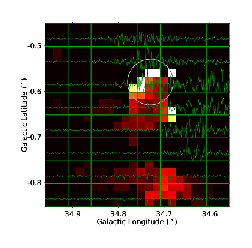
\includegraphics[width = 2.5in]{crrl_eps/G34.7-0.6_ca_spec.eps}}
\subfloat[Infrared color map  ]{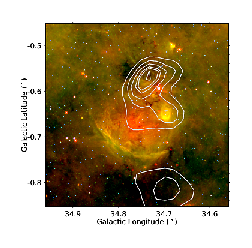
\includegraphics[width = 2.5in]{crrl_eps/G34.7-0.6_rgb_contour.eps}}\\ 
\caption{The C-RRL emission region: G34.7-0.6.
          (a) The SIGGMA spectral grid with the velocity range from $-50$ to 150\kms.
	  The background is the 0$^{th}$ moment C-RRL map over $30$ to $50$\kms.
	  (b) The infrared RGB color map (r: 24\,$\um$, g: 8\,$\um$, b: 4.5\,$\um$) overlaid by integrated RRL contour.
	  The levels are 4, 8, 12, 16, 18, 22 mJy\,beam$^{-1}$\kms.}
\label{fig_crrl-g347}
\end{figure}
\begin{figure}[H]
\centering
\subfloat[SIGGMA spectral grid]{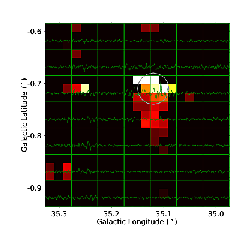
\includegraphics[width = 2.5in]{crrl_eps/G35.1-0.7_ca_spec.eps}}
\subfloat[Infrared color map  ]{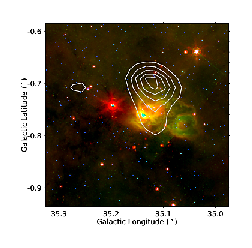
\includegraphics[width = 2.5in]{crrl_eps/G35.1-0.7_rgb_contour.eps}}\\
\caption{The C-RRL emission region: G35.1-0.7.
          (a) The SIGGMA spectral grid with the velocity range from $-50$ to $150$\kms.
	  The background is the 0$^{th}$ moment C-RRL map over $10$ to $40$\kms.
	  (b) The infrared RGB color map (r: 24\,$\um$, g: 8\,$\um$, b: 4.5\,$\um$) overlaid by integrated RRL contour.
	  The levels are 2, 4, 6, 8, 10, 12, 15, 18 mJy\,beam$^{-1}$\kms.}
\label{fig_crrl-g351}
\end{figure}
\begin{figure}[H]
\centering
\subfloat[SIGGMA spectral grid]{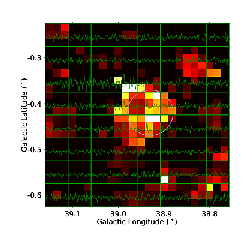
\includegraphics[width = 3.5in]{crrl_eps/G38.9-0.4_ca_spec.eps}}
\subfloat[Infrared color map  ]{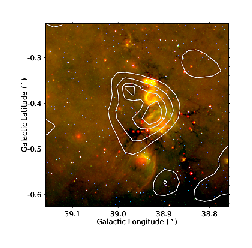
\includegraphics[width = 3.5in]{crrl_eps/G38.9-0.4_rgb_contour.eps}}\\
\caption{The C-RRL emission region G38.9-0.4.
          (a) The SIGGMA spectral grid with the velocity range from $-50$ to $150$\kms.
	  The background is the 0$^{th}$ moment C-RRL map integrated over $20$ to $50$\kms.
	  (b) The infrared RGB color map (r: 24\,$\um$, g: 8\,$\um$, b: 4.5\,$\um$) overlaid with integrated C-RRL contours.
	  The contour levels are 2, 4, 6, 7 mJy\,beam$^{-1}$\kms.}
\label{fig_crrl-g389}
\end{figure}
\begin{figure}[H]
\centering
\subfloat[SIGGMA spectral grid]{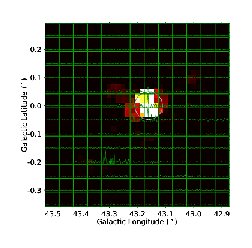
\includegraphics[width = 2.5in]{crrl_eps/G43.2-0.0_ca_spec.eps}}
\subfloat[Infrared color map  ]{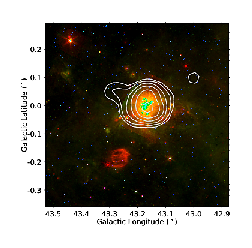
\includegraphics[width = 2.5in]{crrl_eps/G43.2-0.0_rgb_contour.eps}}\\ 
\caption{The C-RRL emission region: G43.2-0.0.
          (a) The SIGGMA spectral grid with the velocity range from $-50$ to $150$\kms.
	  The background is the 0$^{th}$ moment C-RRL map over $-20$ to $20$\kms.
	  (b) The infrared RGB color map (r: 24\,$\um$, g: 8\,$\um$, b: 4.5\,$\um$) overlaid by integrated RRL contour.
	  The levels are 5, 10, 25, 50, 100, 200 mJy\,beam$^{-1}$\kms.}
\label{fig_crrl-g432}
\end{figure}
\begin{figure}[H]
\centering
\subfloat[SIGGMA spectral grid]{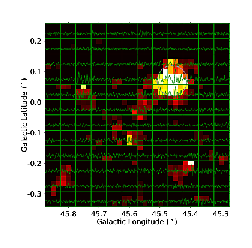
\includegraphics[width = 2.5in]{crrl_eps/G45.5+0.0_ca_spec.eps}}
\subfloat[Infrared color map  ]{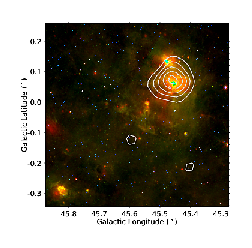
\includegraphics[width = 2.5in]{crrl_eps/G45.5+0.0_rgb_contour.eps}}\\ 
\caption{The C-RRL emission region: G45.5+0.0.
          (a) The SIGGMA spectral grid with the velocity range from $-50$ to $150$\kms.
	  The background is the 0$^{th}$ moment C-RRL map over $30$ to $70$\kms.
	  (b) The infrared RGB color map (r: 24\,$\um$, g: 8\,$\um$, b: 4.5\,$\um$) overlaid by integrated RRL contour.
	  The levels are 5, 10, 15, 20, 25 mJy\,beam$^{-1}$\kms.}
\label{fig_crrl-g455}
\end{figure}
\begin{figure}[H]
\centering
\subfloat[SIGGMA spectral grid]{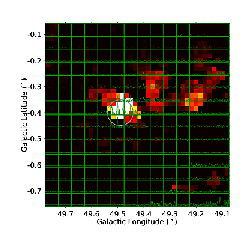
\includegraphics[width = 2.5in]{crrl_eps/G49.5-0.4_ca_spec.eps}}
\subfloat[Infrared color map  ]{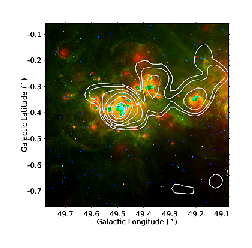
\includegraphics[width = 2.5in]{crrl_eps/G49.5-0.4_rgb_contour.eps}}\\
\caption{The C-RRL emission region: G49.5-0.4
          (a) The SIGGMA spectral grid with the velocity range from $-50$ to $150$\kms.
	  The background is the 0$^{th}$ moment C-RRL map over $30$ to $70$\kms.
	  (b) The infrared RGB color map (r: 24\,$\um$, g: 8\,$\um$, b: 4.5\,$\um$) overlaid by integrated RRL contour.
	  The levels are 5, 10, 25, 50, 100, 200, 250 mJy\,beam$^{-1}$\kms.}
\label{fig_crrl-g494}
\end{figure}
\begin{figure}[H]
\centering
\subfloat[SIGGMA spectral grid]{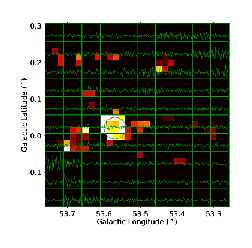
\includegraphics[width = 2.5in]{crrl_eps/G53.6+0.0_ca_spec.eps}}
\subfloat[Infrared color map  ]{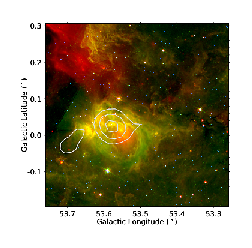
\includegraphics[width = 2.5in]{crrl_eps/G53.6+0.0_rgb_contour.eps}}\\
\caption{The C-RRL emission region: G53.6+0.0
          (a) The SIGGMA spectral grid with the velocity range from $-50$ to $150$\kms.
	  The background is the 0$^{th}$ moment C-RRL map over $0$ to $30$\kms.
	  (b) The infrared RGB color map (r: 24\,$\um$, g: 8\,$\um$, b: 4.5\,$\um$) overlaid by integrated RRL contour.
	  The levels are 2, 4, 6, 8 mJy\,beam$^{-1}$\kms.}
\label{fig_crrl-g536}
\end{figure}
\begin{figure}[H]
\centering
\subfloat[SIGGMA spectral grid]{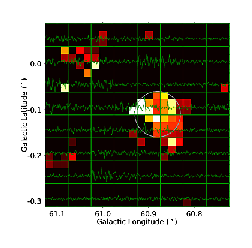
\includegraphics[width = 2.5in]{crrl_eps/G60.9-0.1_ca_spec.eps}}
\subfloat[Infrared color map  ]{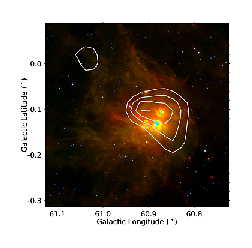
\includegraphics[width = 2.5in]{crrl_eps/G60.9-0.1_rgb_contour.eps}}\\ 
\caption{The C-RRL emission region: G60.9-0.1
          (a) The SIGGMA spectral grid with the velocity range from $-50$ to $150$\kms.
	  The background is the 0$^{th}$ moment C-RRL map over $0$ to $30$\kms.
	  (b) The infrared RGB color map (r: 24\,$\um$, g: 8\,$\um$, b: 4.5\,$\um$) overlaid by integrated RRL contour.
	  The levels are 2, 4, 6, 8 mJy\,beam$^{-1}$\kms.}
\label{fig_crrl-g609}
\end{figure}
\begin{figure}[H]
\centering
\subfloat[SIGGMA spectral grid]{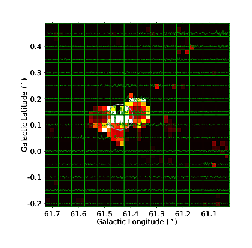
\includegraphics[width = 2.5in]{crrl_eps/G61.4+0.1_ca_spec.eps}}
\subfloat[Infrared color map  ]{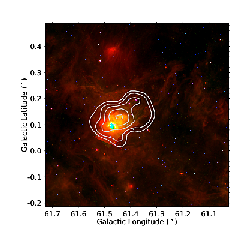
\includegraphics[width = 2.5in]{crrl_eps/G61.4+0.1_rgb_contour.eps}}\\
\caption{The C-RRL emission region: G61.4+0.1
          (a) The SIGGMA spectral grid with the velocity range from $-50$ to $150$\kms.
	  The background is the 0$^{th}$ moment C-RRL map over $0$ to $30$\kms.
	  (b) The infrared RGB color map (r: 24\,$\um$, g: 8\,$\um$, b: 4.5\,$\um$) overlaid by integrated RRL contour.
	  The levels are 5, 10, 20, 40, 80,160, 320 mJy\,beam$^{-1}$\kms.}
\label{fig_crrl-g614}
\end{figure}
\begin{figure}[H]
\centering
\subfloat[SIGGMA spectral grid]{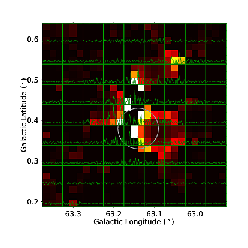
\includegraphics[width = 2.5in]{crrl_eps/G63.1+0.4_ca_spec.eps}}
\subfloat[Infrared color map  ]{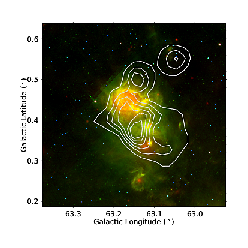
\includegraphics[width = 2.5in]{crrl_eps/G63.1+0.4_rgb_contour.eps}}\\ 
\caption{The C-RRL emission region: G63.1+0.4
          (a) The SIGGMA spectral grid with the velocity range from $-50$ to $150$\kms.
	  The background is the 0$^{th}$ moment C-RRL map over $-5$ to $30$\kms.
	  (b) The infrared RGB color map (r: 24\,$\um$, g: 8\,$\um$, b: 4.5\,$\um$) overlaid by integrated RRL contour.
	  The levels are 5, 10, 15, 20, 25, 30 mJy\,beam$^{-1}$\kms.}
\label{fig_crrl-g631}
\end{figure}

\newpage

\section{Figures of detected H-RRL emission from Galactic Supernova Remnants}\label{appe:snr}

\begin{figure}[H]
\centering
\subfloat[SIGGMA spectral grid]{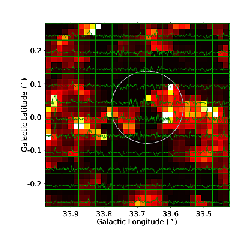
\includegraphics[width = 2.5in]{snr_eps/G33.6+0.1_ha_spec.eps}} 
\subfloat[VGPS 1.4 GHz continuum map]{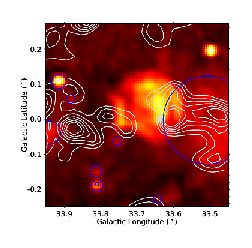
\includegraphics[width = 2.5in]{snr_eps/G33.6+0.1_vgps_contour.eps}}\\  
\caption{The H-RRL emission from SNR: G33.6+0.1.
          (a) The SIGGMA spectral grid with the velocity range from $-300$ to $300$\kms.
	  The background is the 0$^{th}$ moment C-RRL map over $0$ to $150$\kms.
	  The white circle is the central region of the SNR.
	  (b) The VGPS 1.4 GHz continuum map overlaid by integrated RRL contour.
	  The levels are 0.1, 0.15, 0.2, 0.25, 0.3, 0.35 Jy\,beam$^{-1}$\kms.
	  The blue circles are location of \hii\ regions.
	  }
\label{fig_snr-g336}
\end{figure}
\begin{figure}[H]
\centering
\subfloat[SIGGMA spectral grid]{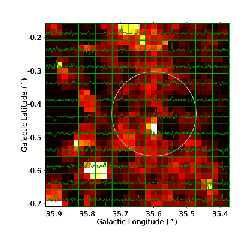
\includegraphics[width = 2.5in]{snr_eps/G35.6-0.4_ha_spec.eps}}
\subfloat[VGPS 1.4 GHz continuum map]{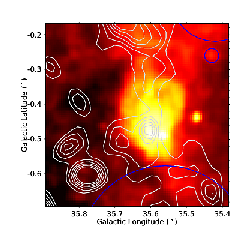
\includegraphics[width = 2.5in]{snr_eps/G35.6-0.4_vgps_contour.eps}}\\
\caption{The H-RRL emission from SNR: G35.6-0.4.
          (a) The SIGGMA spectral grid with the velocity range from $-300$ to $300$\kms.
	  The background is the 0$^{th}$ moment C-RRL map over $0$ to $150$\kms.
	  The white circle is the central region of the SNR.
	  (b) The VGPS 1.4 GHz continuum map overlaid by integrated RRL contour.
	  The levels are 0.05, 0.07, 0.09, 0.11, 0.13, 0.15 Jy\,beam$^{-1}$\kms.
	  The blue circles are location of \hii\ regions.
	  }
\label{fig_snr-g356}
\end{figure}
\begin{figure}[H]
\centering
\subfloat[SIGGMA spectral grid]{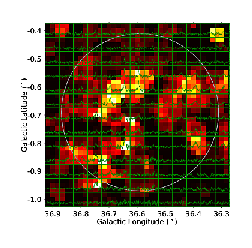
\includegraphics[width = 2.5in]{snr_eps/G36.6-0.7_ha_spec.eps}}
\subfloat[VGPS 1.4 GHz continuum map]{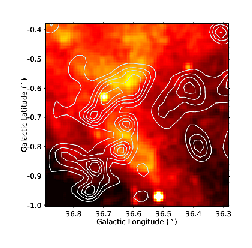
\includegraphics[width = 2.5in]{snr_eps/G36.6-0.7_vgps_contour.eps}}\\
\caption{The H-RRL emission from SNR: G36.6-0.7.
          (a) The SIGGMA spectral grid with the velocity range from $-300$ to $300$\kms.
	  The background is the 0$^{th}$ moment C-RRL map over $0$ to $150$\kms.
	  The white circle is the central region of the SNR.
	  (b) The VGPS 1.4 GHz continuum map overlaid by integrated RRL contour.
	  The levels are 0.04, 0.07, 0.1, 0.13, 0.16 Jy\,beam$^{-1}$\kms.
	  There are no \hii\ regions located in the figure covered region.
	  }
\label{fig_snr-g366}
\end{figure}
\begin{figure}[H]
\centering
\subfloat[SIGGMA spectral grid]{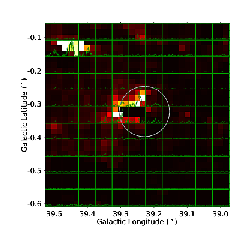
\includegraphics[width = 2.5in]{snr_eps/G39.2-0.3_ha_spec.eps}}
\subfloat[VGPS 1.4 GHz continuum map]{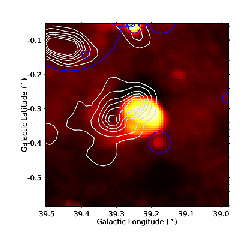
\includegraphics[width = 2.5in]{snr_eps/G39.2-0.3_vgps_contour.eps}}\\
\caption{The H-RRL emission from SNR: G39.2-0.3.
          (a) The SIGGMA spectral grid with the velocity range from $-300$ to $300$\kms.
	  The background is the 0$^{th}$ moment C-RRL map over $0$ to $150$\kms.
	  The white circle is the central region of the SNR.
	  (b) The VGPS 1.4 GHz continuum map overlaid by integrated RRL contour.
	  The levels are 0.1, 0.2, 0.4, 0.6, 0.8, 1.0 Jy\,beam$^{-1}$\kms.
	  The blue circles are location of \hii\ regions.
	  }
\label{fig_snr-g392}
\end{figure}
\begin{figure}[H]
\centering
\subfloat[SIGGMA spectral grid]{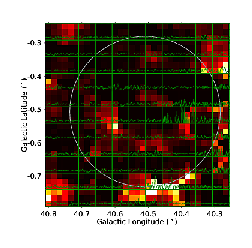
\includegraphics[width = 2.5in]{snr_eps/G40.5-0.5_ha_spec.eps}}
\subfloat[VGPS 1.4 GHz continuum map]{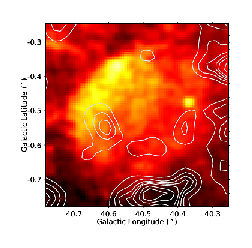
\includegraphics[width = 2.5in]{snr_eps/G40.5-0.5_vgps_contour.eps}}\\
\caption{The H-RRL emission from SNR: G40.5-0.5.
          (a) The SIGGMA spectral grid with the velocity range from $-300$ to $300$\kms.
	  The background is the 0$^{th}$ moment C-RRL map over $0$ to $150$\kms.
	  The white circle is the central region of the SNR.
	  (b) The VGPS 1.4 GHz continuum map overlaid by integrated RRL contour.
	  The levels are 0.02, 0.04, 0.06, 0.08, 0.1, 0.15, 0.2 Jy\,beam$^{-1}$\kms.
	  There are no \hii\ regions located in the figure covered region.
	  }
\label{fig_snr-g405}
\end{figure}
\begin{figure}[H]
\centering
\subfloat[SIGGMA spectral grid]{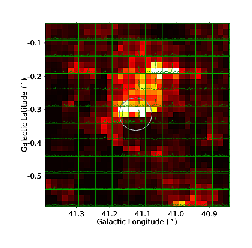
\includegraphics[width = 2.5in]{snr_eps/G41.1-0.3_ha_spec.eps}}
\subfloat[VGPS 1.4 GHz continuum map]{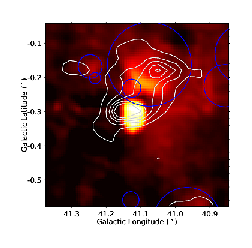
\includegraphics[width = 2.5in]{snr_eps/G41.1-0.3_vgps_contour.eps}}\\
\caption{The H-RRL emission from SNR: G41.1-0.3.
          (a) The SIGGMA spectral grid with the velocity range from $-300$ to $300$\kms.
	  The background is the 0$^{th}$ moment C-RRL map over $0$ to $150$\kms.
	  The white circle is the central region of the SNR.
	  (b) The VGPS 1.4 GHz continuum map overlaid by integrated RRL contour.
	  The levels are 0.1, 0.2, 0.3, 0.4, 0.5 Jy\,beam$^{-1}$\kms.
	  The blue circles are location of \hii\ regions.
	  }
\label{fig_snr-g411}
\end{figure}
\begin{figure}[H]
\centering
\subfloat[SIGGMA spectral grid]{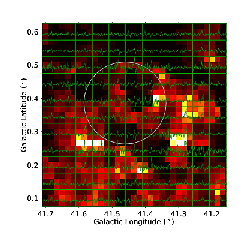
\includegraphics[width = 2.5in]{snr_eps/G41.5+0.4_ha_spec.eps}}
\subfloat[VGPS 1.4 GHz continuum map]{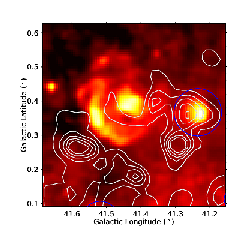
\includegraphics[width = 2.5in]{snr_eps/G41.5+0.4_vgps_contour.eps}}\\
\caption{The H-RRL emission from SNR: G41.5+0.4.
          (a) The SIGGMA spectral grid with the velocity range from $-300$ to $300$\kms.
	  The background is the 0$^{th}$ moment C-RRL map over $0$ to $150$\kms.
	  The white circle is the central region of the SNR.
	  (b) The VGPS 1.4 GHz continuum map overlaid by integrated RRL contour.
	  The levels are 0.05, 0.08, 0.11, 0.14, 0.17 Jy\,beam$^{-1}$\kms.
	  The blue circles are location of \hii\ regions.
	  }
\label{fig_snr-g415}
\end{figure}
\begin{figure}[H]
\centering
\subfloat[SIGGMA spectral grid]{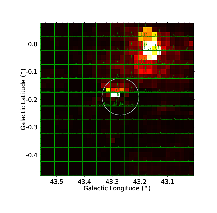
\includegraphics[width = 2.5in]{snr_eps/G43.3-0.2_ha_spec.eps}}
\subfloat[VGPS 1.4 GHz continuum map]{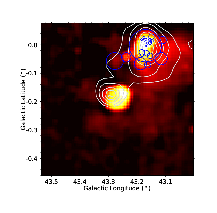
\includegraphics[width = 2.5in]{snr_eps/G43.3-0.2_vgps_contour.eps}}\\
\caption{The H-RRL emission from SNR: G43.3-0.2.
          (a) The SIGGMA spectral grid with the velocity range from $-300$ to $300$\kms.
	  The background is the 0$^{th}$ moment C-RRL map over $0$ to $150$\kms.
	  The white circle is the central region of the SNR.
	  (b) The VGPS 1.4 GHz continuum map overlaid by integrated RRL contour.
	  The levels are 0.25, 0.5, 1, 1.5, 2, 2.5, 3 Jy\,beam$^{-1}$\kms.
	  The blue circles are location of \hii\ regions.
	  }
\label{fig_snr-g433}
\end{figure}
\begin{figure}[H]
\centering
\subfloat[SIGGMA spectral grid]{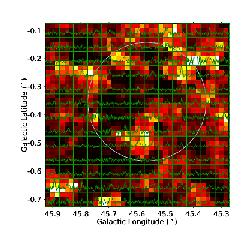
\includegraphics[width = 2.5in]{snr_eps/G45.7-0.4_ha_spec.eps}}
\subfloat[VGPS 1.4 GHz continuum map]{
\includegraphics[width = 2.5in]{snr_eps/G45.7-0.4_vgps_contour.eps}}\\
\caption{The H-RRL emission from SNR: G45.7-0.4.
          (a) The SIGGMA spectral grid with the velocity range from $-300$ to $300$\kms.
	  The background is the 0$^{th}$ moment C-RRL map over $0$ to $150$\kms.
	  The white circle is the central region of the SNR.
	  (b) The VGPS 1.4 GHz continuum map overlaid by integrated RRL contour.
	  The levels are 0.05, 0.1, 0.15, 0.2, 0.25, 0.3, 0.4 Jy\,beam$^{-1}$\kms.
	  The blue circles are location of \hii\ regions.
	  }
\label{fig_snr-g457}
\end{figure}
\begin{figure}[H]
\centering
\subfloat[SIGGMA spectral grid]{\includegraphics[width = 2.5in]{snr_eps/G46.8-0.3_ha_spec.eps}}
\subfloat[VGPS 1.4GHz continuum map]{\includegraphics[width = 2.5in]{snr_eps/G46.8-0.3_vgps_contour.eps}}\\
\caption{The H-RRL emission from SNR: G46.8-0.3.
          (a) The SIGGMA spectral grid with the velocity range from $-300$ to $300$\kms.
	  The background is the 0$^{th}$ moment C-RRL map over $0$ to $150$\kms.
	  The white circle is the central region of the SNR.
	  (b) The VGPS 1.4 GHz continuum map overlaid by integrated RRL contour.
	  The levels are 0.1, 0.15, 0.2, 0.25, 0.3, 0.4 Jy\,beam$^{-1}$\kms.
	  The blue circle is the location of a \hii\ region.
	  }
\label{fig_snr-g468}
\end{figure}
\begin{figure}[H]
\centering
\subfloat[SIGGMA spectral grid]{\includegraphics[width = 2.5in]{snr_eps/G49.2-0.7_ha_spec.eps}}
\subfloat[VGPS 1.4GHz continuum map]{\includegraphics[width = 2.5in]{snr_eps/G49.2-0.7_vgps_contour.eps}}\\
\caption{The H-RRL emission from SNR: G49.2-0.7.
          (a) The SIGGMA spectral grid with the velocity range from $-300$ to $300$\kms.
	  The background is the 0$^{th}$ moment C-RRL map over $0$ to $150$\kms.
	  The white circle is the central region of the SNR.
	  (b) The VGPS 1.4 GHz continuum map overlaid by integrated RRL contour.
	  The levels are 0.5, 1, 1.5, 2, 2.5, 3, 3.5, 4 Jy\,beam$^{-1}$\kms.
	  The blue circles are location of a \hii\ regions.
	  }
\label{fig_snr-g492}
\end{figure}
\begin{figure}[H]
\centering
\subfloat[SIGGMA spectral grid]{\includegraphics[width = 2.5in]{snr_eps/G54.4-0.3_ha_spec.eps}}
\subfloat[VGPS 1.4GHz continuum map]{\includegraphics[width = 2.5in]{snr_eps/G54.4-0.3_vgps_contour.eps}}\\
\caption{The H-RRL emission from SNR: G54.4-0.3.
          (a) The SIGGMA spectral grid with the velocity range from $-300$ to $300$\kms.
	  The background is the 0$^{th}$ moment C-RRL map over $0$ to $150$\kms.
	  The white circle is the central region of the SNR.
	  (b) The VGPS 1.4 GHz continuum map overlaid by integrated RRL contour.
	  The levels are 0.05, 0.15, 0.25, 0.35, 0.45 Jy\,beam$^{-1}$\kms.
	  The blue circles are location of a \hii\ regions.
	  }
\label{fig_snr-g544}
\end{figure}
\begin{figure}[H]
\centering
\subfloat[SIGGMA spectral grid]{\includegraphics[width = 2.5in]{snr_eps/G57.2+0.8_ha_spec.eps}}
\subfloat[VGPS 1.4GHz continuum map]{\includegraphics[width = 2.5in]{snr_eps/G57.2+0.8_vgps_contour.eps}}\\
\caption{The H-RRL emission from SNR: G57.2+0.8.
          (a) The SIGGMA spectral grid with the velocity range from $-300$ to $300$\kms.
	  The background is the 0$^{th}$ moment C-RRL map over $0$ to $150$\kms.
	  The white circle is the central region of the SNR.
	  (b) The VGPS 1.4 GHz continuum map overlaid by integrated RRL contour.
	  The levels are 0.03, 0.05, 0.07, 0.09 Jy\,beam$^{-1}$\kms.
	  There are no \hii\ regions located in the figure covered region.
	  }
\label{fig_snr-g572}

\end{figure}

\newpage

\bibliography{siggmaii}
\bibliographystyle{aasjournal}

\end{document}


